\documentclass{article}
\title{Using Monte Carlo Bootstrapping to analyse the conflicts of assumption violations in polynomial regression.\\}
\author{Christian, Jonathan, Marcus, Puk \& Sofia }
\date{28\textsuperscript{th} May 2025}


\usepackage[utf8]{inputenc}
\usepackage[T1]{fontenc}
\usepackage{xcolor}

\usepackage{graphicx}
\usepackage{epstopdf}
\usepackage{booktabs}
\usepackage[hidelinks]{hyperref}
\usepackage{amsmath}
\usepackage[content={}, color=white]{background}


\definecolor{aaublue}{rgb}{0.129,0.102,0.322}
\definecolor{codegreen}{rgb}{0,0.6,0}
\definecolor{codegray}{rgb}{0.5,0.5,0.5}
\definecolor{codepurple}{rgb}{0.58,0,0.82}
\definecolor{backcolour}{rgb}{0.95,0.95,0.92}
\usepackage{listings}
\lstdefinestyle{mystyle}{
	backgroundcolor=\color{backcolour},
	commentstyle=\color{codegreen},
	keywordstyle=\color{magenta},
	numberstyle=\tiny\color{codegray},
	stringstyle=\color{codepurple},
	basicstyle=\ttfamily\footnotesize,
	breakatwhitespace=false,
	breaklines=true,
	captionpos=b,
	keepspaces=true,
	numbers=left,
	numbersep=5pt,
	showspaces=false,
	showstringspaces=false,
	showtabs=false,
	tabsize=2,
	language=R 
}
\lstset{style=mystyle} 


\usepackage{graphicx}
\usepackage{epstopdf} 
\usepackage{booktabs}
\usepackage{amsmath}
\usepackage[hidelinks]{hyperref} 

\begin{document}
	
	
	\setcounter{section}{0}
	\pdfbookmark[0]{Front page}{label:frontpage}%
\thispagestyle{empty} 
\begin{titlepage}
\vspace*{\fill}
    \backgroundsetup{
    scale=1.2,
    angle=0,
    opacity=1.0,  %% adjust
    contents={
\includegraphics[width=\paperwidth,height=\paperheight]{media/aau_waves.pdf}}
    }
  \addtolength{\hoffset}{0.5\evensidemargin}
  \addtolength{\hoffset}{-0.5\oddsidemargin}
  %set equal margins on the frontpage - remove this line if you want default margins
  \noindent%
  {\color{white}\fboxsep0pt\colorbox{aaublue}{\begin{tabular}{@{}p{\textwidth}@{}}
    \begin{center}
    \Huge{\textbf{
       Using Monte Carlo Bootstrapping to analyse the conflicts of assumption violations in polynomial regression}}\\
      % insert your title here
    \end{center}
    \vspace{0.2cm}
   \begin{center}
    {\Large
      Data Science and Machine Learning - Spring 2025 - Ccs-25-dvml-2-02 % insert name of study, group number, year-month
    }
   \end{center}
%% Comment this section in if you are doing Bachelor or Master Project   
   \begin{center}
    {\Large
     2. Semester Project
      %Bachelor Project
      \vspace{0.5cm}
    }
   \end{center}
  \end{tabular}}}
  \vfill
  \begin{center}
    %
\includegraphics[width=0.2\paperwidth]{AAUgraphics/aau_logo_circle_en}% comment this line in for English version
    
\includegraphics[width=0.2\paperwidth]{media/aau_logo_circle_en} %comment this line in for Danish version
  \end{center}
\end{titlepage}
\clearpage

	
\phantomsection
\pdfbookmark[0]{Titlepage}{titlepage}
\thispagestyle{empty}
%\thispagestyle{plain}
\setcounter{page}{1} %sidetallet starter først her fra
\begin{minipage}[t]{0.48\textwidth}
\vspace*{-25pt}			%\vspace*{-9pt}

\includegraphics[height=4cm]{media/aau_logo_en.pdf}
\end{minipage}
\hfill
\begin{minipage}[t]{0.48\textwidth}
{\small 

Department of Computer Science \\
Selma Lagerløfs Vej 300 \\
Aalborg Ø, 9220 \\
\url{http://www.es.aau.dk}}
\end{minipage}

\vspace*{1cm}

\begin{minipage}[t]{0.48\textwidth}
\textbf{Title:} \\[5pt]\hspace*{2ex}
\noindent Using Monte Carlo Bootstrapping to Analyse the Conflicts of Assumption Violations in Polynomial Regression

\vspace*{2ex}

\textbf{Project:} \\[5pt]\bigskip\hspace{2ex}
2. Semester Project

\textbf{Period:} \\[5pt]\bigskip\hspace{2ex}
Februar 2025 -  May 2025

\textbf{Group:} \\[5pt]\bigskip\hspace{2ex}
cs-25-dvml-2-02

\textbf{Members:} \\[5pt]\hspace*{2ex}
Christian Filtenborg Brogaard \\\hspace*{2ex}
Jonathan Skovbjerg Karoff \\\hspace*{2ex}
Marcus Lundgaard Terndrup \\\hspace*{2ex}
Puk Thejlmann Kalstrup \\\hspace*{2ex}
Sofia Jean Sabbah \\\hspace*{2ex}


\textbf{Associated professors:} \\[5pt]\hspace*{2ex}\\
Tomer Sagi, Deparment of Computer Science
\\\hspace*{2ex}

\vspace*{1cm}

\textbf{Pages: ?????} \\
%\textbf{Appendices: XXX to XXX} \\
\textbf{Handed in ?????}

\end{minipage}
\hfill
\begin{minipage}[t]{0.5\textwidth}
\textbf{Abstract}: \\[5pt]
\fbox{\parbox{8cm}{Regression models are powerful tools for drawing statistical inferences from data. They serve as a gateway to more advanced statistical analysis and inference. However, despite their power, regression models are also quite fragile. This fragility stems from the assumptions that must be satisfied in order to avoid misleading or invalid conclusions. In this project we will focus on the effects of Monte Carlo Bootstrapping and how it can be used to overcome assumption violations, specifically violation in the assumption of homoscedasticity. We determine the effects of Monte Carlo Bootstrapping by resampling synthetic data, that contains multicollinearity. Two polynomial regression models are then created: one utilizing the resampled data and the other derived from the original data. The two models are compared in metrics such as root mean squared error and mean bias error. We conclude that the polynomial regression model derived from resampled data, has a greater accuracy. }}
\end{minipage}

\vfill

{\footnotesize\itshape \noindent The content of the report is freely available, but publication (with source reference) may only take place in agreement with the authors.}

% Rapportens indhold er frit tilgængeligt, men offentliggørelse (med kildeangivelse) må kun ske efter aftale med forfatterne.
% The content of the report is freely available, but publication (with source reference) may only take place in agreement with the authors.

	\newpage
	\tableofcontents
	\newpage
	
	\section{Introduction}
	
Regression is a tool in statistics used to understand the relationship between one dependent variable and one or more independent variables. For regression to be both accurate and reliable, a set of assumptions needs to be met. These assumptions are independence of errors, linearity, homoscedasticity, normality of errors, multicollinearity, and correct model specifications. If these assumptions are not met, it can introduce bias and inaccuracies in the regression model.
	\newpage
	
	\section{Problem Analysis}
	Collecting data is nothing new. Information is gathered in the form of samples, or collections of observations. Samples are collected from populations, which are collections of all individuals or individual items of a particular type. At times a population signifies a scientific system; other times it is represented as the rest of society. When conducting a data analysis, we aim to identify relationships in society, in other words, to estimate the parameters of the population. While collecting data is one step, analysing it and drawing meaningful conclusions is a much more complex task. To help make these decisions and draw conclusions, inferential statistics are used. \cite{ProbAndStat} Specifically, fitting a regression model to data based on a sample and making predictions based on the model about the population. \newline

\noindent The central problem when regression models are fitted to data is to determine the true relationship among the variables. The problem is that the true relationship is not known, and we have to depend upon the sample observations to estimate the true relationship. In this case, the chosen regression model should be able to generalise beyond the sample data. \newline 



\subsection{Assumptions for Regression Models}

\noindent Regression models are tools for understanding relationships between variables. However, for this to work, certain assumptions need to be satisfied. This section will briefly explain the previously mentioned key assumptions that are essential to ensure reliable results and the ability to predict beyond the sample. It is still possible to create regression models without these assumptions, but it becomes undeniably harder.  \newline

\noindent The first assumption is called Independence of Errors, and it states that the errors from the model are not correlated with each other, they are independent. This means that one error cannot be used to predict the next one. \newline


\noindent The next is the assumption of Linearity, which states that the relationship between the independent variables and the parameters, also known as the coefficients, is linear. This does not mean that the regression model itself has to be linear. For example, in polynomial regression, the relationship between the independent variables and the coefficients is still linear, but the independent variables can be transformed using powers.\newline


\noindent Then there is Homoscedasticity, which is, as mentioned, the assumption of constant variance across errors for all levels of the independent variables. This assumption will be addressed in more detail later. \newline

\noindent Next, is the assumption, Normality of Errors which states that the errors between the model and the observed values, also called residuals, are normally distributed. If this is not met, it may result in a biased model and a worse model fit. \newline


\noindent Then, there is the assumption of Multicollinearity which occurs when two or more independent variables in a regression model are highly correlated with each other. This means that changes in one independent variable are associated with changes in another, making it difficult to determine the individual effect of each independent variable on the dependent variable. \newline

\noindent Last assumption is Correct Model Specifications which assume that the provided dependent variables for the models are the correct ones. If one is missing, or the model is overfitting, this may result in incorrect coefficients and introduce errors into the model. \newline
 
These are the key assumptions when it comes to regression models. But, the mentioned assumptions are not guaranteed when working with empirical data. 
 

\subsection{Empirical Data}
To give an example of empirical data containing assumption violations is the "Miles Per Gallon" data set. Using the dataset it is possible to model the assumption violations, as seen in \autoref{fig:1} and \autoref{fig:2}.
\newline

\begin{figure}
	\centering
	\centering
	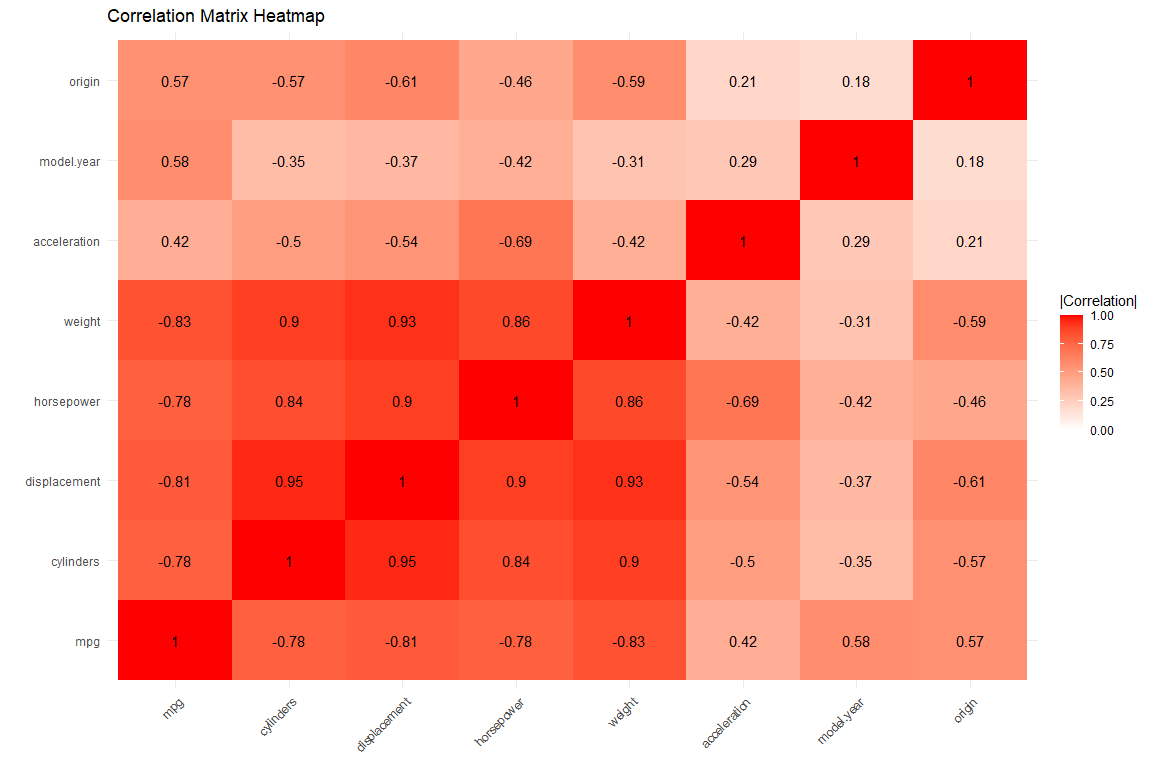
\includegraphics{billder/1.png}
	\caption{Heatmap made from the MPG dataset}
	\label{fig:1}
\end{figure}

\noindent The first assumption violation is multicollinearity, which can be seen in Figure 1. It means, per earlier definition, that independent variables in the dataset are highly correlated with each other. Therefore, it becomes more difficult to isolate the individual effect of each variable, if a regression model was fitted to the data.
In \autoref{fig:1} it is shown through the numbers, where the high numbers suggest a strong linear relationship between the variables. So, for example looking at the variables, 'displacement' and ' cylinders', the value is 0.95. Since it is close to 1, it shows that there is multicollinearity. \newline


\begin{figure}[h]
	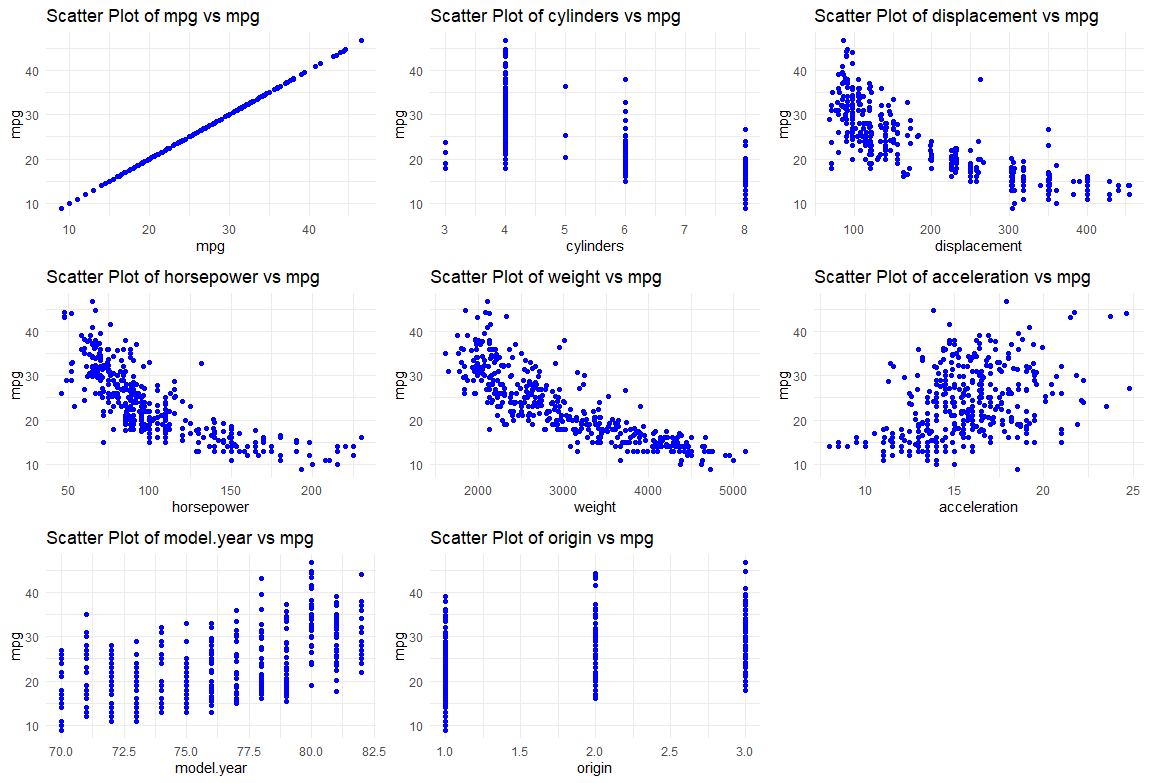
\includegraphics[width=\linewidth]{billder/2.png}
	\caption{Scatterplots made from the MPG dataset}
	\label{fig:2}
\end{figure}
\noindent The next assumption violation seen in the dataset is homoscedacticity. Looking at \autoref{fig:2} there is an example of hetereoscedasticity in the scatterplot of the variables 'mpg' and 'horsepower'. There is clearly not constant variance of the residuals in that scatterplot, because there is a big spread between the variables when horsepower decreases. \newline

\noindent So, it shows that data does not always adhere to these assumptions, and the results may be inaccurate if the assumption violations are not accounted for. \newline

\noindent To understand how the classical method of constructing regression models and the method of using Monte Carlo Bootstrapping works, we need to dive deeper into the background. Here, we need to understand ways to not only create a model, but how to test it as well. These topics will be explained in the following section.


	\newpage
	
	\section{Real world data example}
	Noticing if assumptions are not met is important when looking at data from real life.
To understand how breached assumptions look when modeled, looking at realistic data becomes necessary. \newline

(heatmap)
Multicollinearity can be seen in this heatmap made from the MPG dataset. Multicollinearit occurs when independent variables are highly correlated with each other, and as a result, it becomes more difficult to isolate the individual effect of each variable in a regression model.
In this model it is shown through the numbers, where the high numbers suggest a strong linear relationship through the variables. So between 'displacement' and ' cylinders', the value is 0.95, which is close to 1 and therefore shows there is multicollinearity. \newline

(scatterplot)
Here is an example of hetereoscedasticity in the 'mpg' and 'horsepower' scatterplot, where there is not constant variance of the residuals. This is seen because there is a big spread between the variables, especially when horsepower decreases.   

	\newpage
	\section{Background}
	her Puk :)
	\subsection{Statistical theory}
	This section will focus on the theoretical background needed to understand how to create regression models, how to test a models reliability and significance, how to generate data and how Monte Carlo Bootstarpping works.

\noindent Sections 3.1 through 3.5 are based on the book 'Probability and Statistics for Engineers and Scientists' \cite{ProbAndStat}. \newline

\noindent Statistics is a field in mathematics, that gives tools to analyze and understand data. Statistics comes in two branches, these are descriptive statistics and inferential statistics. Descriptive statistics is used to describe the general tendencies in some data, such as finding the mean and variance, but no predictions or conclusion are made beyond the data itself. In contrast, inferential statistic is the branch of statistics that makes predictions and generalizations of a population based on a sample, this includes methods such as hypothesis testing and regressions. 

\noindent To address the challenges, when violations in the assumptions of modeling regressions through classical means occur, a fundamental statistical understanding is needed. This section introduces the foundational concept of statistics that is required to understand regression models.


\subsection{Probability space}

The \textbf{sample space}, \textit{S}, is the set of all possible outcomes.
\newline
If a sample space contains a finite number of possibilities or an unending sequence with as many elements as there are whole numbers, it is called a \textbf{discrete sample space}.
\newline
Example: When rolling a standard six-sided die form the discrete sample space, the possible outcomes are $S={1,2,3,4,5,6}$ 
\newline

If a sample space contains an infinite number of possibilities equal to the number of points on a line segment, it is called a \textbf{continuous sample space}.
\break
Example: Measuring the heights of people in a population. This is a continuous sample space, because height can take any real value within a given range. 
\newline
An \textbf{event} is a subset, $A\subseteq S$, of the sample space. The event is the amount that contains all possible events.
An example of a discrete event could be rolling a die and getting an uneven number, this would be the event $A={1,3,5}$.
\newline 
For the continuous event, it could be that a person is between 160 cm and 170 cm tall.
\newline

The probability of an event \textit{A}, $P(A)$, is the sum of the weights of all sample points in \textit{A}.
The probability of the whole sample space is 1, $P(S)=1$
The probability of any event being between 0 and 1,$0<P(A)<1$
The probability of the empty set being 0, $P(Ø)=0$
\newline
\newline
Probability of mutually exclusive events
\newline
If \textit{A} and \textit{B} are mutually exclusive, $A \cap B=Ø$, then
\newline
$P(A \cup B) = P(A)+P(B)$
\newline
\newline
Where \textit{A} and \textit{B} never occur at the same time, so their union is equal to the two events added together. 
\newline
Probability of union
\newline
$P(A \cup B)=P(A)+P(B)-P(A \cap B)$
\newline
Here, the union of the two events is \textit{A} added to \textit{B}, but minus their common event, since it otherwise would be added twice. 
\newline
Two events \textit{A} and \textit{B} are independent, if 
\newline
$P(A|B)=P(A)$
\newline
The equivalent definition to this is:
\newline
Two events \textit{A} and \textit{B} are independent if and only if 
\newline
$P(A \cap B)=P(A)P(B)$
This says that the probability of both event \textit{A} and \textit{B} happening, is equal to the product of the two events.


\subsection{Random Variables}
Now we will introduce random variables, which are important to understand when analysing assumption violations. In statistics, data and results can vary. To understand and handle this randomness, we use random variables, to help describe this uncertainty. \newline

\noindent A random variable is defined as a function that associates a real number with each element in the sample space. We use capital letters to denote a random variabel, for example $X$, and then the corresponding small letter, in this case $x$, for one of its values. As an example we roll a dice 3 times, which gives us a sample space of the different combinations. Each point in the sample space gets a numerical value assigned between 0 and 3.For example, if the random variabel $X$ assumes the number of 5's rolled, then worst case is zero 5's rolled, and best case is three 5's rolled. These values are random quantities assumed by the random variabel $X$, and they are written like this: $X(5,1,2) = 1$ and $X(3,6,1) = 0$.
\newline

\noindent A random variable $X$ can be discrete, which means that its set of possible outcomes is countable. The dice example is a discrete random variable, because you can count how many times 5 is rolled. The outcomes of some statistical experiments may be neither finite nor countable. For example when something is measured such as temperature or speed where the set of possible values is an entire interval of numbers, it is not discrete. The random variable $X$ then takes values on a continues scale, which therefore is called a continuous random variable.

\subsubsection{Discrete Random Variable}
\label{sec:disc}
A discrete random variable can take each of its values with a certain probability. Frequently, it is convenient to represent all the probabilities of a random variable $X$ by a formula. Let $X$ be a discrete random variable which can take the values $x_{1}, x_{2},...$ Then the distribution of $X$ is given by the probability function:

\begin{equation}
	f(x_{i})=P(X=x_{i}),\quad i=1,2,...
\end{equation}
\newline
For a discrete random variable this function is also called the probability mass function, where following holds for each possible outcome $x$:

\begin{itemize}
	\item $P(X = x) = f(x).$
	\item $f(x) \geq 0,$
	\item $\sum_x f(x) = 1.$
\end{itemize}

\noindent In addition to the probability mass function $f$, the discrete random variable $X$ also has a cumulative distribution function $F(x)$ given by:

\begin{equation}
F(x) = P(X \leq x) = \sum_{x_i \leq x} f(x_i), \quad x \in \textbf{R}.
\end{equation}


\noindent This helps decide the probability that the random variable assumes a value equal to or smaller than $x$. Its sums up the probability density functions values.
\newline

\noindent The mean of a discrete variable $X$, with a distribution function $f(x_{i})$ is given by:

\begin{equation}
\mu = E(X) = \sum_i x_i P(X = x_i) = \sum_i x_i f(x_i).
\end{equation}

\noindent The mean is typically the expected value. It is a weighed average of the possible values of $X$. The values are weighed by its probability in the sample space.
\\

\noindent In addition to the mean, we should also mention the variance. The variance is the mean squared distance between the values of the variable and the mean value. It is given by:

\begin{equation}
\sigma^2 = E\left[(X - \mu)^2\right] = \sum_{i} (x_i - \mu)^2 f(x_i)
\end{equation}

\noindent The variance indicates whether the values of $X$ are far from the mean values or close. A high variance means that the values of $X$ have a high probability of being far from the mean values and vice versa. Along with the variance, the standard deviation is also often used. It is given by the square root of the variance:
\begin{equation}
\sigma=+\sqrt{\sigma^2}.
\end{equation}

\noindent The advantage of the standard deviation over the variance is that it is measured in the same units as $X$.

\subsubsection{Continuous Random Variable}
Contrary to a discrete random variable, a continuous random variable can take values that are not countable. A continuous random variable can take infinetly many possible values within a certain range or interval. For a continuous random variable $X$ the distribution is given by the probability density function $f$, which satisfies:

\begin{itemize}
	\item $f(x)$ is defined for all $x$ in $\textbf{R}$,
	\item $f(x) \geq 0$ for all $x$ in $\textbf{R}$,
	\item $\int_{-\infty}^{\infty} f(x) \, dx = 1.$
\end{itemize}

\noindent Condition 3. ensures that $P(-\infty < X < \infty) = 1$, which means that the probability of the random variable $X$ being between $-\infty$ and $\infty$ is 100\%. Furthermore the probability of $X$ assuming a specific value $a$ is zero, in other words: $P(X=a)=0$. That means that the values of the density function should not be interpreted as a probability of a given outcome. Instead the probability of $X$ is found by integrating over the probability density function. So, the probability that a continuous random variable $X$ lies between the values $a$ and $b$ is: 

\begin{equation}
P(a < X < b) = \int_a^b f(x) \, dx.
\end{equation}


\noindent A continuous random variable $X$ also has a distribution function $F(x)$, that also predicts whether $X$ assumes a value equal to or smaller than $x$. For a continuous random variable it is again given by integrating over the probability density function in the interval from $-\infty$ to $x$:
\begin{equation}
F(x) = P(X \leq x) = \int_{-\infty}^{x} f(y) \ dy.
\end{equation}


\noindent That also means $P(a<X<b)$ can be calculated by $F(b)-F(a)$.
\\

\noindent For a continuous random variabel $X$ the mean, variance and standard deviation the same interpretation applies. Just given by different formulars, which are:
\begin{equation}
	\mu = E(X) = \int_{-\infty}^{\infty} x f(x) \, dx
\end{equation}

\noindent and
\begin{equation}
\sigma^2 = E\left[(X - \mu)^2\right] = \int_{-\infty}^{\infty} (x - \mu)^2 f(x) \, dx,
\end{equation}

\noindent (The standard deviation is still given by til square root of the variance).


\subsection{Estimator and estimates}
If we are interested in certain parameters of a population distribution, we can look at a sample. From this, we can make a point estimate. 
\newline
Examples of this are, 
\newline
$\bar{x}$ is a point estimate of $\mu$
\newline
s is a point estimate of $\sigma$
\newline

\noindent This is often supplemented with a confidence interval.
\newline
This is an interval around the point estimate, where we are confident that the population parameter is located.
\newline

\noindent For $\mu$, we have different ways of estimating it. We can use the sample mean $\bar{X}$, or the average $X_T$ of the sample upper and lower quartiles. 
But in this case, we have to look out for bias. If the distribution of a population is skewed, then $X_T$ is biased. The result of this is, that in the long run, this estimator will systematically over or under estimate the value of $\mu$. This is written as,
\newline
$E(X_T) \neq \mu$.
\newline
It is generally preferred that the estimator is unbiased. In this case, $\bar{X}$ is an unbiased estimate of the population mean $\mu$.
\newline

\noindent The standard error of $\bar{X}$ is $\frac{\sigma}{\sqrt{n}}$. Here, the standard error decreases, when the sample size increases. If an estimator has this property, it is called consistent. If we compare, the estimator $X_T$ is also consistent, but has a greater variance than $\bar{X}$. 
\newline
It is generally preferred that the estimator has the smallest possible variance, and in that case it is called efficient. So $\bar{X}$ is an efficient estimator.
\newline
When estimating a parameter, the symbol $\hat{}$ is used above it. For $\mu$, $\hat{\mu} = \bar{X}$ .
\newline
We can calculate $\bar{X}$ using the following formula,
$$\bar{X}=\frac{1}{n} \sum_{i=1}^{n}X_i$$   
\newline
For the variance $\sigma$, we can estimate it by using the formula for $S^2$,
$$S^2=\frac{1}{n-1} \sum_{i=1}(X_i-\bar{X})$$
\subsection{Probability distribution}
Data can come in various distributions depending on different parameters such
as degrees of freedom. The distribution is the shape of the data and it will have
an effect on statistical models. Therefore it is important to have an understanding of distributions.
\subsubsection{Normal distribution}
In the world of statistics, the most common distribution is the normal distribution. It is constructed as a bell shape. The normal distribution is a continuous distribution, with this density function:
$$n(x;\mu,\sigma) =\frac{1}{\sqrt{2\pi\sigma}}e^{-\frac{(x-\mu)}{2\sigma^2}}$$
The distribution is dependent on the mean($\mu$) and the standard deviation($\sigma$), where changes to the mean will result in a change in the positioning of the normal distribution. Whereas a change in the standard deviation will change the spread of the curve. The normal distribution also always contains an area under the curve that is equal to one. This is to ensure that the normal distribution correctly models probability.

There is a special case of the normal distribution, called the standard normal distribution, where the mean is zero and the standard deviation is one. All variations of a normal distribution can be standardized by a transformation of the distribution, using the Z-score formula.
\newline
$$Z=\frac{X-\mu}{\sigma}$$
\newline
$Z$ in the Z-score represents the amount of standard deviations a given $X$ value, deviates from the mean.

\subsubsection{The central limit theorem}
A very effective theorem in statistics is the central limit theorem. This theorem states that if a random sample $\overline{X}$, with the size $n$, is taken from a population with a mean and a finite variance, then as $n$ goes towards infinity, the distribution will resemble a normal distribution. If used with the Z-score formula, the distribution will resemble a standard normal distribution. The formula for the Z-score, when in conjunction with the central limit theorem, looks like this:
$$Z=\frac{\overline{X}-\mu}{\sigma/\sqrt{n}}$$
Where $\overline{X}$ is a random sample of size $n$ and $\mu$ is the mean of the true population. The standard error i represented by $\sigma/\sqrt{n}$, where $\sigma$ is the standard deviation and $n$ is the sample size.
Usually the standard deviation is unknown, for these situations it's possible to use the estimator $S^2$. This estimates the variance of the population from the variance of the sample, by this formula:
$$s^2=\sum_{i=1}^{n}\frac{(x_{i}-\overline{x})}{n-1}$$

The square root of the variance is the standard deviation, therefore the square root of the estimator $S^2$ would be the estimated standard deviation. The problem with using the estimator $S^2$, is that with small samples the variance is small and therefore it contains a lot of bias. In this situation the t-distribution would be used instead of the normal distribution, because the t-distribution takes the bias into account the bias of the standard deviation. It does this by having thicker tails, meaning that the probability of more extreme values are higher.

\subsubsection{The t-distribution}
The t-distribution is shaped as the standard normal distribution, in a bell shape and symmetrical around the mean of zero, the difference is that the t-distribution is more variable. This comes from the fact that the t-distribution is dependent on the degrees of freedom. When the degrees of freedom surpasses 30, the rule of thumb is that the distribution will resemble a normal distribution. So before 30 degrees of freedom, the distribution contains more variance.
The t-distribution will come to resemble the standard normal distribution, when in surpasses 30 degrees of freedom, this makes sense, since the two distributions have the same formula:
$$T=\frac{\overline{X}-\mu}{S/\sqrt{n}}$$

The only difference is the estimated standard deviation $S$.
\newpage
\subsection{Statistical methods}

\subsubsection{Confidence intervals}
The confidence interval is a good tool to use, when trying to estimate a parameter of a population. Its used to create an interval, where the parameter has a probability to lie inside of. This probability is called the confidence level and it's a chosen value, usually the chosen confidence level is either 95\% or 99\%. The confidence interval will become bigger with a larger confidence level. A good confidence interval is small with a large confidence level, this will usually occur when the sample size is large. The chosen confidence level relates to an $\alpha$-value, where as an example the chosen confidence level is 95\%, then the $\alpha$-value would be 5\% or normally written as $0.05$. The $\alpha$-value will sometimes be needed to find the critical value, that is used to calculate the margin of error, as an example it's used when trying to find the critical value of the confidence interval, when working with a t-distribution.
\newline
To set up a confidence interval, the margin of error needs to be computed and then that will be both added and subtracted from the point estimate. This will give the values of the outer bounds of the interval. The margin of error is calculated from this formula:
$$Margin\_of\_error = critical\_value \pm standard\_error$$
\newline
The standard error will change depending on which parameter that the confidence interval is estimating, but the general formula for the standard error is:
$$\frac{\sigma}{\sqrt{n}}$$
\newline
An example of computing a confidence interval of the mean while working with a standard normal distribution, then the formula for the confidence interval would be this:

$$P(-z_{\alpha/2}<Z<z_{\alpha/2}) = 1-\alpha$$
\newline
Where $1-\alpha$ is the confidence level. As it's the mean that is being estimated, then instead of Z-score, then $\mu$ must be isolated and that is done by multiplying $\frac{\sigma}{\sqrt{n}}$ and subtracting $\bar{X}$ on all sides, then multiplying all side by $-1$ to remove the minus sign. So the formula for a confidence interval of the mean will look like this:

$$P(\bar{X}-z_{\alpha/2}\frac{\sigma}{\sqrt{n}}<\mu<\bar{X}+z_{\alpha/2}\frac{\sigma}{\sqrt{n}})=1-\alpha$$
\newline
This formula will give the upper and lower bounds of the confidence interval.\\

\noindent \textbf{The interpretation of a confidence interval}
\newline
To interpret a confidence interval, it would be incorrect to interpret the confidence level of some value $x$, as the probability of the true parameter being inside of the interval. The reason behind this is that the computed interval is static, so either the value $x$ is inside the interval or it's not. So the correct way of interpreting the confidence interval is by taking multiple samples and computing the confidence interval for all samples, then the value $x$ would reside inside 95\% of the confidence intervals.
\textbf{Kilde for fortolkningen af kofidense intervaller:}
\newline
$http://www.drhuang.com/science/mathematics/book/probability_and_statistics_for_engineering_and_the_sciences.pdf$


\subsubsection{Hypothesis testing}
A hypothesis test is used to test an assumption about a population. This is done from a sample of the population, as the information about the population is usually hard to come by. A hypothesis test is set up, by having a null hypothesis and an alternate hypothesis.
$$H_0 = Null\; hypothesis$$
$$H_a = Alternate\; hypothesis$$
When working with hypothesis testing, the hypothesis $H_0$ is usually represented as the status quo, where as the hypothesis $H_a$ is represented as the opposition. It is also important to note that there is only two outcomes of a hypothesis test, either $H_0$ is rejected in favor of $H_a$ or $H_0$ is failed to be rejected. Therefore in no situation can $H_0$ be stated to be an absolute truth, as there might be other samples where $H_0$ will be rejected. Therefore in a hypothesis test $H_0$ needs to be the thing that can be rejected and if $H_0$ gets rejected, then $H_a$ will become the new status quo until proven otherwise.\\
In a hypothesis test $H_0$ will be the assumption that a parameter for two populations is the same, where as $H_a$ can be either one of three assumptions, depending on the intention of the hypothesis test.
$$H_0: \theta = \theta_0$$
$$1.\;H_a: \theta \neq \theta_0$$
$$2.\;H_a: \theta < \theta_0$$
$$3.\;H_a: \theta > \theta_0$$
When the direction of the rejection is not important and also is unknown, then (1) will be the case. This scenario sets up a two-tailed-test, where the hypothesis test is used to reject $H_0$ if $H_a$ is either significantly larger or smaller than $H_0$, this means that the critical area is on both sides of the difference of $\theta$ and $\theta_0$. Either (2) or (3) will set up a one-tailed-test, where depending on what is important, either the hypothesis test is used to determine if $H_a$ is significantly bigger or smaller than $H_0$. This means that the critical area only spans one side of the difference between $\theta$ and $\theta_0$.\\

\newline
\noindent \textbf{Error in hypothesis testing}
\newline
When making a hypothesis test there is four different possible outcomes. The results are separated by correct decisions and errors. There exist two types of hypothesis errors, called type 1 error and type 2 error. The type 1 error occurs when $H_0$ is mistakenly rejected and $H_0$ is true. Type 2 error is the opposite, where $H_a$ is rejected and $H_a$ is true. The types of outcomes occurring from a hypothesis test can be seen in Table \ref{tab:example2x3}
\begin{table}[h!]
	\centering
	\begin{tabular}{|c|c|c|}
		\hline
		 & $H_0$ is true & $H_0$ is false \\
		\hline
		Does not reject $H_0$ & Correct decision & Type 2 error \\ \hline
		Reject $H_0$ & Type 1 error & Correct decision \\
		\hline
	\end{tabular}
	\caption{Outcomes of a hypothesis test}
	\label{tab:example2x3}
\end{table}

It is possible to compute the possibility of a type 1 error occurring, because the probability is equal to the significance level also denoted as $\alpha$. So when a significance level of 0.05 is chosen, then that is the same as the probability of a type 1 error occurring. As for computing the probability of a type 2 error occurring, it can only be done if $H_a$ is defined. The probability of a type 2 error occurring is denoted as $\beta$ and by a defined $H_a$, whats meant is that the $\mu$ of the sample is needed. Depending on the distribution and sample size, the calculation of $\beta$ will change.
As an example in a normal distributed sample, the $\mu$ is needed in calculating a Z-score and this Z-score is needed to extract a value from the Z-table. Then the probability of a type 2 error occurring is calculated from this formula:
$$
\beta = 1-\phi(Z_\beta)
$$
In this formula $\phi(Z_\beta)$ is the value from the Z-table. Its possible to reverse this formula and denote the probability of a correct decision, where $H_0$ is rejected and $H_a$ is true, this is denoted as, $1-\beta$.
It is possible to change the probability of these two errors occurring, this is done by changing the significance level. The consequence of this is that one of the errors will always lower its probability of occurring, while the other will have its probability increased. By reducing the significance level, the type 1 error will have a lower probability of happening, but a type 2 error will have an increase in probability of occurring. The opposite where the significance level is increased, the probability of the type 1 error will increase and for the type 2 error, it will be reduced. To overcome this problem, the only solution is to increase the sample size, as this will lower the probability of either of the two error types of happening.





	\newpage
	\subsection{Polynomial regression}
	\subsection{Regression Model}
Understanding the relationship between variables is crucial when working with data, as it forms the basis for drawing meaningful conclusions. Regression models are a fundamental statistical tool used to model and analyse these relationships. In this project the chosen model, we are working with is polynomial regression. This section will explain the neccessary theory to understand this model. It will also explain assumption violations in more detail. Specifically the assumption of constant variance of errors also called homoscedasticity and the assumption of no multicollinearity.

\subsubsection{Regression}
Sections $4.6.1$, $4.6.2$ and $4.6.3$ are based on the book 'Applied Lienar Statistical Models' \cite{AppliedLSM}. 
\newline 

\noindent Before looking at polynomial regression, we have to understand linear regression. \newline 
Linear regression is a model that estimates the relationship between a dependent variable, \( Y \), and one or more independent variables, \( x \). A reasonable relationship between the two in simple regression is the linear relationship:
\begin{equation}
Y = \beta_0 + \beta_1 x .
\end{equation}


\noindent Where \( \beta_0 \) is the intercept, and \( \beta_1 \) is the slope.

\noindent In a lot of cases, there will be more independent variables, so the relationship for multiple regression will look like this:

\begin{equation}
	Y = \beta_0 + \beta_1 x_1 + ......+ \beta_n x_n .
\end{equation}




\noindent Where \( n \) is the number of independent variables, and $\beta_2$ further shapes the curvature and complexity of the curve. A widely used method to determine the parameters of linear models is the least square method, in order to find the best fitting line for the data.

\noindent In simple linear regression, the random error \( \epsilon \) is included:
\begin{equation}
Y = \beta_0 + \beta_1 x + \epsilon .
\end{equation}


\noindent It is assumed that \( \epsilon \) is distributed with $\epsilon = 0$ and $\epsilon = \sigma^2$, and it has consistent variance, which is usually called the Homogeneous Variance Assumption. The random error \( \epsilon \) adds randomness to account for the natural variability in real data, making the model more realistic.
\newline\\
Polynomial regression is a form of linear regression, but the relationship between \( x \) and \( Y \) is an \( n \)th-degree polynomial. It fits a nonlinear relationship between the value of \( x \) and the corresponding conditional mean of \( Y \), meaning the model predicts the expected value of \( Y \) given \( x \). \newline

\noindent That is why it is used when the relationship between the independent variable and the dependent variable is better represented by a curve rather than a straight line, since it can show the nonlinear patterns in the data.
In polynomial regression, as mentioned earlier, there are six assumptions, that should be met, for the model to be as accurate as possible.


\subsubsection{The Method of Least Squares}

\noindent To find connections in data, it is necessary to estimate coefficients, $\beta_0$ and $\beta_1$, in linear models. 
A widely used method to estimate the coefficients, is the previously mentioned least squares method, which will be referred to as Ordinary Least Squares or OLS in the rest of the project. \newline

\noindent OLS considers the deviation of $Y_i$ for  its expected value, where the observations are $(X_i, Y_i)$. 
This method also requires, that we consider the sum of the $n$ squared deviations.
This is denoted by the criterion $Q$,
\begin{equation}
Q=\sum_{i=1}^{n}(Y_i-\beta_0 - \beta_1 X_i)^2 .
\end{equation}

\noindent According to the method of OLS, the estimations of $\beta_0$ and $\beta_1$ that minimize Q for the given sample observations $(X_1,Y_1), (X_2,Y_2), ..., (X_n,Y_n)$, are called $b_0$ and $b_1$.  

\noindent If an analytical approach is used, the values $b_0$ and $b_1$ that minimize Q for any particular set of sample data are given by these simultaneous equations: 
\begin{equation}
\sum Y_i =n b_0 +b_1 \sum X_i ,
\end{equation}

\begin{equation}
\sum X_i Y_i = b_0 \sum X_i + b_1 \sum X_1^2 .
\end{equation}

\noindent These equations are called $normal equations$, where $b_0$ and $b_1$ are the $point estimators$ of $\beta_0$ and $\beta_1$. It is possible to calculate these normal equations simultaneously for $b_0$ and $b_1$ through these expressions,

\begin{equation}
b_1 = \frac{\sum (X_1 - \bar{X}) (Y_i - \bar{Y})}{\sum (X_i - \bar{X})^2} ,
\end{equation}

\begin{equation}
	b_0 = \frac{1}{n} (\sum Y_i - b_1 \sum X_i ) = \bar{Y} - b_1 \bar{X} .
\end{equation}

\noindent Here, $\bar{X}$ and $\bar{Y}$ are the means of $X_i$ and $Y_i$. The normal equations can also be derived by differentiating with respect to $\beta_0$ and $\beta_1$:

\begin{equation}
	\frac{\partial Q}{\partial \beta_0}=-2 \sum (Y_i - \beta_0 - \beta_1 X_i) ,
\end{equation}
\begin{equation}
\frac{\partial Q} {\partial \beta_1} = -2 \sum X_i (Y_i - \beta_0 - \beta_1 X_i) .
\end{equation}

\noindent By setting these derivatives equal to zero, we can find $b_0$ and $b_1$, 

\begin{equation}
	-2 \sum (Y_i - b_0 - b_1 X_1)=0 ,
\end{equation}
\begin{equation}
	-2\sum X_i(Y_i - b_0 - b_1 X_1)=0 .
\end{equation}

\noindent This can be simplified, 
\begin{equation}
\sum_{i=1}^{n} (Y_i - b_0 - b_1 Xi)=0£ ,
\end{equation}
\begin{equation}
	\sum_{i=1}^{n} X_1(Y_i - b_0 - b_1 Xi)=0£ .
\end{equation}
And it can be expanded, so the normal equations are obtained, 

\begin{equation}
	\sum Y_1 - n b_0 - b_1 \sum X_1 =0 ,
\end{equation}

\begin{equation}
	\sum X_1 Y_1  - b_0 \sum X_1 - b_1 \sum X_i^2 =0 .
\end{equation}

\noindent Solving this for $b_0$ and $b_1$ will lead to values, that minimize Q, and these are the estimates for $\beta_0$ and $\beta_1$. 
When rearranging terms, we get the normal equations $(28)$ and $(29)$. The estimates $b_0$ and $b_1$ obtain the minimum when checking the second partial derivatives. \newline


\subsubsection{Linear Models}
Equations for linear models can be written in matrix terms, where the normal error regression model for simple linear regression is.
 

\begin{equation}
Y_i = \beta_0 + \beta_1 X_i 0 \epsilon_i .
\end{equation}


\noindent Which implies that,

\begin{equation}
Y_1 = \beta_0 + \beta_1 X_1 + \epsilon_1
\end{equation}

\begin{equation}
Y_2 = \beta_0 + \beta_1 X_2 + \epsilon_2
\end{equation}
$$\vdots$$
\begin{equation}
Y_n = \beta_0 + \beta_1 X_n + \epsilon_n .
\end{equation}

\noindent The observations vector $Y$ is,
\begin{equation} Y_{n \times 1} =
\left[
\begin{array}{c}
	Y_1 \\ 
	Y_2 \\ 
	\vdots \\
	Y_n 
\end{array}
\right].
\end{equation}

\noindent The X matrix is, 

\begin{equation}X_{n \times 2}=
\left[
\begin{array}{cc}
	1 & X_1 \\ 
	1 & X_2 \\ 
	\vdots & \vdots \\
	1 & X_n
\end{array}
\right].
\end{equation}


\noindent The $\beta$ vector is, 
\begin{equation}\beta_{2 \times 1} =
\left[
\begin{array}{c}
	\beta_0 \\ 
	\beta_1 
\end{array}
\right].
\end{equation}

\noindent And the $\epsilon$ vector is,
\begin{equation} \epsilon_{n \times 1} =
\left[
\begin{array}{c}
	\epsilon_0 \\ 
	\epsilon_1 \\
	\vdots \\
	\epsilon_n 
\end{array}
\right].
\end{equation}

\noindent This can be written in matrix terms with a dot product, 
\begin{equation} Y_{n \times 1}=X_{n \times 2} \cdot \beta_{2 \times 1} + \epsilon_{n \times 1} ,
\end{equation}

\noindent where, \newline
\textbf{$Y$} is a vector of response \newline
\textbf{$\beta$} is a vector of parameters \\
\textbf{$X$} is a matrix of constants, called det design matrix\\
\textbf{$\epsilon$} is a vector of independent normal random variables with expectation\\

\noindent This can be shown in columns,
\begin{equation}
\left[
\begin{array}{c}
	Y_1 \\ 
	Y_2 \\ 
	\vdots \\
	Y_n 
\end{array}
\right]
=
\left[
\begin{array}{cc}
	1 & X_1 \\ 
	1 & X_2 \\ 
	\vdots & \vdots \\
	1 & X_n
\end{array}
\right]
\left[
\begin{array}{c}
	\beta_0 \\ 
	\beta_1 
\end{array}
\right]
+
\left[
\begin{array}{c}
	\epsilon_0 \\ 
	\epsilon_1 \\
	\vdots \\
	\epsilon_n 
\end{array}
\right].
\end{equation}

\noindent If the dependent variable $Y$ has more than one independent variable in a linear model, the equation looks like this, 

\begin{equation} Y_i = \beta_0 + \beta_1 X_{i1} + \beta_2 X_{i2} + ... + \beta_p-1 X_{i, p-1} + \epsilon_i .
\end{equation}

\noindent In matrix terms it is,  
\begin{equation}
\left[
\begin{array}{c}
	Y_1 \\ 
	Y_2 \\ 
	\vdots \\
	Y_n 
\end{array}
\right]
=
\left[
\begin{array}{cccc}
	1 & X_{11} & ... & X_{1, p-1} \\ 
	1 & X_{21} & ... & X_{2, p-1} \\ 
	\vdots & \vdots &  & \vdots \\
	1 & X_{n1} & ... & X_{n, p-1}
\end{array}
\right]
\left[
\begin{array}{c}
	\beta_0 \\ 
	\beta_1 \\
	\vdots \\
	\beta_p-1 
\end{array}
\right]
+
\left[
\begin{array}{c}
	\epsilon_0 \\ 
	\epsilon_1 \\
	\vdots \\
	\epsilon_n 
\end{array}
\right].
\end{equation}

\noindent The $Y$ and $\epsilon$ vectors are the same as in the simple linear regression matrix. The $\beta$ vector has additional parameters, and the $X$ matrix now has a column of $n$ observations for each $p-1 X$ variables. 

\subsubsection{Polynomial Regression}
Polynomial regression models the relationship like this, 
\begin{equation}
	Y=\beta_0 + \beta_1 x + \beta_2 x^2	+ ... + \beta_{p-1} x^{p-1}+ \epsilon .
	\end{equation}

\noindent The coefficients can still be found through the method of least squares,

\begin{equation}
	Q=\sum_{i=1}^{n}(Y_i -(\beta_0 + \beta_1 X_i + \beta_2 x_i^2 + ... + \beta_{p-1}X_{i}^{p-1}))^2 .
\end{equation}
\newline

\noindent This can be written in matrix terms as,
\begin{equation}
	Q=(Y-X\beta)' (Y-X\beta). 
\end{equation}

\noindent Where the design matrix for polynomial regression is, 

\begin{equation}
	 X=
\left[
\begin{array}{ccccc}
	1&x_1&x_1^2&...&x_1^{p-1}\\ 
	1&x_2&x_2^2&...&x_2^{p-1} \\
	\vdots & \vdots &\vdots &&\vdots\\
	1&x_n&x_n^2&...&x_n^{p-1} 
\end{array}
\right].
\end{equation}

\noindent We can expand the expression from before, so it looks like this,
\begin{equation}
	Q=Y' Y -Y' X \beta -\beta' X' Y + \beta' X' X \beta .
\end{equation}


\noindent It is possible to find the value of $\beta$ that minimizes Q by differentiating with respect to $\beta_0$ and $\beta_1$,

\begin{equation}
\frac{\partial}{\partial \beta}(Q)=
\left[
\begin{array}{c}
	\frac{\partial Q}{\partial \beta_0}\\ 
	\frac{\partial Q}{\partial \beta_1}
\end{array}
\right].
\end{equation}

\begin{equation}
\frac{\partial}{\partial \beta}(Q)=-2 X' Y + 2X' X \beta .
\end{equation}

\noindent Then minimum is found by calculating, where the gradient is 0.
\begin{equation}\b-2 X' Y+ 2X' X \beta =0,\end{equation}
\begin{equation} 2X' X \beta = 2X' Y,\end{equation}
\begin{equation}(X' X)^{-1} X' X \beta = (X' X)^{-1} X' Y,\end{equation}
\begin{equation} \beta=(X' X)^{-1} X' Y.\end{equation}
  For this to be calculated, the matrix $X' X$ has to be invertible, so the columns of $X$ have to be linearly independant.
 
 \noindent So, 
 
\begin{equation}
 	X' Xa  =0
\end{equation}
\begin{equation}
 	a' X' X a =0
\end{equation}
\begin{equation}
 	(Xa)'(Xa)=0
\end{equation}
 
 \noindent This shows, that $X'Xa=0$ if and only if $(Xa)'(Xa)=0$, so $Xa=0$. 
 
 \noindent If it is supposed, that there exists a non-trivial solution for $Xa=0$, there also exists a non-trivial solution for $X'Xa=0$. It is therefore only invertible when the null space of $X$ is 0, or if the columns are linearly independent. 
 
\noindent To ensure that the solution gives a minimum, the hessian matrix is calculated,
\begin{equation}
 \frac{\partial^2 Q}{\partial \beta' \beta}=2X'X.
\end{equation} 
 \noindent If it is positive definite, the function Q has a global minimum, which can be shown with,
\begin{equation}
 a' (X' X)a = (Xa)' (Xa).
\end{equation}  
 \noindent As shown in $(63)$,
 these can only be calculated coefficients, if $Xa \not= 0$. This means, that $X'X$ is positive definite in all relevant situations, which is when the coefficients can be calculated. 
 
 \noindent The solution to the least squares method results in only containing $X'X$ and $X'Y$.
 The matrices are,
 
 
\begin{equation}
 X=
 \left[
 \begin{array}{ccc}
 	1 &X_1	& X_1^2\\ 
 	1 & X_2 & X_2^2	\\
 	\vdots & \vdots & \vdots \\
 	1 & X_n& X_n^2
 \end{array}
 \right],
\end{equation}
 
 \begin{equation}
 	X'X=
 \left[
 \begin{array}{ccccc}
 	n &\sum X_i	& \sum X_i^2 & ... &\sum X_i^{p-1}\\ 
 	\sum X_i & \sum X_i^2 & \sum X_i^3&...& \sum X_i^p	\\
 	\sum X_i^2 & \sum X_i^3 & \sum X_i^4 & ... & \sum X_i^{p+1}\\
 	\vdots&\vdots&\vdots& & \vdots	\\
 	\sum X_i^{p-1} &\sum X_i^p& \sum X_i^{p+1} & ... & \sum X_i^{2p-2}
 \end{array}
 \right],
\end{equation}
 
 \begin{equation}
 	X' Y=
 \left[
 \begin{array}{c}
 	\sum Y_i\\ 
 	\sum X_i Y_i	\\
 	\sum X_i^2 Y_i \\
 	\vdots	\\
 	\sum X_i^{p-1} Y_i
 \end{array}
 \right].
\end{equation}
 
 \noindent These are the necessary matrices to use the least squares method.

	\subsubsection{Assumptions}
	When making a regression its important to understand, that the regression has assumptions that needs to be fulfilled if the statistical conclusions are to be correct. If these assumptions are not upheld, it will create bias that will skew the results of the model.
\subsubsubsection{Homoscedasticity}
One of the assumptions of a polynomial regression is that homoscedasticity is fulfilled. Homoscedasticity is the assumption of constant error variance, where observations in a dataset would exhibit errors that have roughly the same spread across all levels of the independent variable.
\newline
If this assumption is not upheld, then this will cause the standard error to be biased and therefore not trustworthy. This problem causes further testing involving this standard error to become wrong, an example is the hypothesis test.
\newline
The reason for the assumption needs to be upheld, comes from how the regression is created. The regression is created via the ordinary least square method, that requires the assumption of homoscedasticity to be upheld.
\newline
A way to display homoscedasticity is through the variance-covariance matrix. The matrix shows whether the data contains homoscedasticity or heteroscedasticity through the diagonal values, that is the variance for the error in each independent variable in the regression. The variances in the matrix are calculated through an alternate equation from the one presented in \autoref{sec:disc}.
\begin{equation}
	\text{Var}(X) = \frac{1}{n - 1} \sum_{i=1}^{n} (x_i - \bar{x})^2
\end{equation}
The equation differs in that it excludes the weighting function and it assumes equal probability for each data point. These changes stems from the data deriving from a sample rather than the population. Consequently the use of $\frac{1}{n-1}$ rather than $\frac{1}{n}$, is to account for the bias correction. This correction is essential, as it prevents underestimation when working with samples rather than populations, by addressing bias.\\
If the matrix contains approximately the same values through the diagonal, then the assumption of homoscedasticity is upheld, else the data contains heteroscedasticity. This is a showcase of the variance-covariance matrix with homoscedasticity:


	
\begin{equation}
Var(\varepsilon) = \mathbb{E}[\boldsymbol{\epsilon} \boldsymbol{\epsilon}'] = 
\left[
\begin{array}{cccc}
	\sigma^2 & 0        & \cdots & 0 \\
	0        & \sigma^2 & \cdots & 0 \\
	\vdots   & \vdots   & \ddots & \vdots \\
	0        & 0        & \cdots & \sigma^2 \\
\end{array}
\right]
\end{equation}


\noindent The general way of writing the variance-covariance matrix, when the mean of the error i assumed to be $0$, is by this formula:
\begin{equation}
Var(\varepsilon) = \mathbb{E}[\boldsymbol{\epsilon} \boldsymbol{\epsilon}'] = 
\left[
\begin{array}{cccc}
	\sigma^2_{11} & \sigma_{21} & \cdots & \sigma_{i1} \\
	\sigma_{12} & \sigma^2_{22} & \cdots & \sigma_{i2} \\
	\vdots      & \vdots      & \ddots & \vdots      \\
	\sigma_{1j} & \sigma_{2j} & \cdots & \sigma^2_{ij}
\end{array}
\right]
\end{equation}

\noindent Every position in the matrix is calculated, then the diagonal will tell if the data contains homoscedasticity or heteroscedasticity. The off-diagonal values represent covariances between error terms. While not the focus of this project, non-zero values here may indicate correlation between errors, which would violate the assumption of independence \cite{Heteroscedasticity} . \newline 

\noindent \textbf{Detecting Heteroscedasticity} \\
When working with data, one method of checking for heteroscedasticity is to visualize it through plotting the residuals, but its not always possible to detect heteroscedasticity through visual media. Another approach is to calculate if the data contains heteroscedasticity. This can be done through the Breusch-Pagan test, that is specifically designed to detect heteroscedasticity. The test detects heteroscedasticity, by regressing the residuals on the independent variables and checks if the independent variables have an effect on the residual variance. If this is not the case, then there is no heteroscedasticity. This checked through a hypothesis test, where the $H_0$ is that the data contains homoscedasticity and $H_a$ is that the dataset contains heteroscedasticity \cite{HomoSce}.

\subsubsubsection{No Multicollinearity}
Perfect multicollinearity is a term used for describing a perfect linear relationship between two or more independent variables. This relationship occurs when an independent variable can be perfectly predicted from other independent variables. In mathematical terms, this could be written as a linear regression:
\begin{equation}
X_1 = \alpha+\beta_1\cdot X_2+...+\beta_n\cdot X_n
\end{equation}
Where $X_1...X_n$ is all the independent variables that have a perfect linear relationship. The coefficients are represented by $\beta_1...\beta_n$ and they are the amount that $X_1$ changes when their relative independent variable changes.
Lastly $\alpha$ is the intercept and represents the value of $X_1$, when all other independent variables are zero.
\newline
The regression model can feel the effects of multicollinearity even without there being perfect multicollinearity. A strong linear relationship is enough to have an effect on the model. The problem caused by multicollinearity, is that as it increases the variance of the value that the coefficients can receive also increases. Where as perfect multicollinearity will make the model unable to estimate a value of one coefficient, due to the perfect linearity between the independent variables \cite{MultAndMis}.
\newline

\noindent \textbf{Detecting Multicollinearity}\\
A common method to detect multicollinearity in a dataset, is to compute the pearson´s correlation coefficient for all combinations of independent variables. This will result in the correlation matrix, as seen in \autoref{fig:1}, where each cell represents the strength and direction of the relationship between two independent variables. The Pearsons correlation coefficient is calculated through this formula:
\begin{equation}
r = \frac{n \sum xy - (\sum x)(\sum y)}{\sqrt{[n \sum x^2 - (\sum x)^2][n \sum y^2 - (\sum y)^2]}}
\end{equation}
Where $n$ is the number of observations, with $x$ and $y$ representing the two variables tested for correlation and the pairwise correlation coefficient is denoted as $r$. When computing the value of $r$, the value will be in a range: $-1\leq r \leq 1$. If the value of $r$ is $-1$ or $1$, that indicates a perfect either negative or positive correlation and if the value is $0$, then there is no correlation between the variables. The correlation matrix has a connection to the variance-covariance matrix, by the correlation matrix being a normalized version of the variance-covariance matrix. This means that for each spot in the variance-covariance matrix, the value is divided by the product of the standard deviations of the corresponding independent variables. By normalizing the values, then the values will go from $-1$ to $1$.\cite{DetectMulti} \newline


\noindent\\\\
To test the consequences of violating the assumption of multicollinearity, a metric to determine model complexity is needed. This is because a more complex model, given the same parameters plus an additional one, will always be more accurate than the same model with fewer parameters. The question of model complexity is too large for the scope of this assignment. Therefore, the consequences of violating the assumption of multicollinearity will not be further investigated. Instead, we will focus on the consequences of violating the assumption of homoscedasticity. \newline



	\newpage
	\subsection{PRNG}
	When producing a synthetic dataset, there is a need for a lot of random numbers. Many programming languages have a built-in function that produces numbers that appear random, but actually are not. Computers are deterministic machines, and therefore cannot produce a number without some sort of algorithm. If the algorithm is known, it becomes possible to predict the next number; hence the numbers are not completely random. Random numbers should be independent; that is, each number should have no connection to any previously produced values. The distribution should also be uniform, meaning if you generate 1,000,000 random numbers in the range [0,1), you'd expect about 500,000 values in [0, 0.5) and about 500,000 in [0.5, 1). Earlier in history, these numbers have been produced by flipping coins or rolling dice. Today, it is possible to produce truly random numbers by using atmospheric noise. Despite its potential advantages, this method requires significant resources, making it inefficient for the intended application. Therefore, pseudo-random numbers will be used instead.
\newline

\noindent Pseudo-random numbers behave like random numbers but are deterministically generated from a seed value. While
these numbers are not truly random, they are sufficiently unpredictable for many practical applications.
To generate the data, we use a Pseudo-Random Number Generator (PRNG).
PRNGs are algorithms that produce sequences of numbers that appear random.
\newline

\noindent Random numbers are widely used in fields such as statistics, game theory, cryptography, and simulations. These applications require numbers that behave
as if they were random, yet can be reproduced when needed. This is where
PRNGs come in. They allow for repeatable randomness, making them ideal for
controlled experiments, testing, and security.
\\
This chapter will explore the key concepts behind PRNGs. Before going into the
mechanics of these generators, it is important to first understand what ’random’
means and the characteristics that define truly random numbers.

\subsection{Properties of PRNGs}

The quality of a PRNG is determined by several key factors that influence its
use for different applications. Some of the properties of a good PRNG are independence, a long period and reproducibility
\newline \\
The numbers produced by the PRNG should be statistically independent, en-
suring that each generated value exhibits no correlation with previous numbers
or other sequences. This implies that knowledge of previously generated num-
bers or sequences provides no advantage in predicting the next output.
\newline \\
A PRNG operates within a specific interval before its sequence begins to repeat.
A high-quality PRNG has a long interval, delaying repetition and enhancing its
unpredictability. Conversely, a PRNG with a shorter period becomes more pre-
dictable and less suitable for practical use.
\newline \\
A key feature of a PRNG is its ability to reproduce the same sequence of num-
bers when given a specific seed. This property is particularly useful in testing
and simulation scenarios, where it is essential to generate identical sequences
multiple times for consistency and reproducibility.
\newline \\
In addition, a PRNG must be fast and efficient to prevent it from introducing
performance bottlenecks within an application. The speed of number generation
directly impacts computational efficiency, especially in applications requiring a
large volume of random numbers. An inefficient PRNG can significantly slow
down processes, undermining the overall performance of the system. Therefore,
balancing randomness and efficiency is essential for practical applications

\subsection{Linear Congruential Generator}

Linear Congruential Generator (LCG) is a commonly used approach to generate
pseudo-random numbers. LCG generates a sequence of numbers using a linear
recurrence relation, expressed as:

$$X_{n+1} = (aX_n + c) \bmod m.$$  \\
\\
\noindent $X_0$ is the seed value and must be in the range $0 \leq X_0 < m$ \newline
$a$ is the multiplier,\newline 
$c$ is the increment and \newline
$m$ is the modulus, which specifies the range of values. $m$ must be greater than 0 \newline
\\
\noindent The operation 'mod $m$' represents division by $m$, where only the remainder
is retained. This ensures that the generated number remains within the range
0 to $m-1$.  $X_0$, $a$ and $c$ must all be in the interval $[0, m)$. 
Here is an example of the first 4 numbers of a sequence given these parameters: \newline

\begin{center}
	$a = 5$, $c = 1$, $m = 16$, and $X_0 = 7$:
\end{center}

$$X_1 = (5 \cdot 7 + 1)\bmod 16 = 4 $$
$$X_2 = (5 \cdot 4 + 1) \bmod 16 = 5 $$
$$X_3 = (5 \cdot 5 + 1) \bmod 16 = 10 $$
$$X_4 = (5 \cdot 10 + 1) \bmod 16 = 3 $$
\\
\noindent This sequence has a period of 16. In an LCG, the period can be as large as $m$,
because the remainder after division by $m$ will always be less than or equal to
$m$. Consequently, choosing a large $m$ is typically desirable, as it can potentially
lead to longer periods. However, the period length is not determined solely by
$m$; the choice of other parameters—such as the multiplier, increment, and the
seed, along with their relationships, significantly impact the overall period. It
is possible to select a larger $m$ and still end up with a shorter period if the parameters are not chosen properly. Here is an example where a larger $m$ results in a shorter period, illustrating that.

\begin{center}
	$a=4$, $c=6$, $m=20$, $X_0=3$
\end{center}

$$X_1=(4 \cdot 3 +6)=18 \bmod 20=18$$ 
$$X_2=(4 \cdot 18+6)=78 \bmod 20=78 \bmod 20=18$$

\noindent Here a larger $m$ is used, but a shorter period of 1 appears. 
\newline \\
The selection of the optimal parameters for a LCG would be excessive for the objective of this project, it is beyond the scope of this project and will therefore not be addressed further.

\subsection{Test of PRNG}
As stated previously, the length of the sequence produced by the PRNG is not the only important factor. A uniform distribution and independence of each generated number is significant too. If these criteria are not met, there will be correlation between the generated numbers, which means that the randomness is of low quality. For example, consider a sequence that follows the three-times-table, with the first number being 3: (3,6,9,12,...). In that sequence, it is pretty easy to guess the upcoming number, based on the previous one. Normally the correlations are harder to spot than this example, which is why it is important to test the quality of a PRNG.
\newline

\noindent There are different tests used to evaluate PRNG quality and performance, including the Kolmogorov-Smirnov test, chi-squared test and the spectral test. Passing one of these tests does not mean that it will pass others. Therefore, every test that it passes, just makes it more likely to produce a high quality sequence. One of the important tests for LCG is the spectral test. Another advantage of the spectral test in the context of this paper is that it can be visualized in two or three dimensions, which can make it easier to understand.
\newline

\noindent The test looks at how the numbers in the sequence are distributed in different dimensions. If hyperplanes and lines occur, as seen on Figure \ref{fig:badspec2d} and Figure \ref{fig:badspec3d}, generated by $X_{n+1}=137\cdot X_{n}+187$ mod $256$, the sequence fails the test, since the distribution is not random.
\newline

\noindent Looking at the spectral test used on a LCG with better parameters:  $X_{n+1}=3 141 592 621\cdot X_{n}+1$ mod $2^{32}$ (Kilde: Knuth), on Figure \ref{fig:goodspec2d} and Figure \ref{fig:goodspec3d}, the hyperplanes will not always be visible in 2d or 3d, but only in higher dimensions. Therefore a visual examination will not be enough to conclude the complete quality of a PRNG. Methods for inspecting LCGs in these dimensions do exist, but will not be mentioned in this project
\newline

\noindent In this project, the PRNG used will be the Mersenne-Twister. It has very good properties, uniformity and a period of $2^19937-1$ and passes the spectral test. The test in 2D and 3D can be seen on figure \ref{fig:msspec2d} and figure \ref{fig:msspec3d}. Another reason for this choice is that Mersenne-Twister is the built-in generator in R, which makes it convenient. 
\newpage

%Spectral test for bad LCG
\begin{figure}
	\centering
	\begin{minipage}{0.45\textwidth}
		\centering
		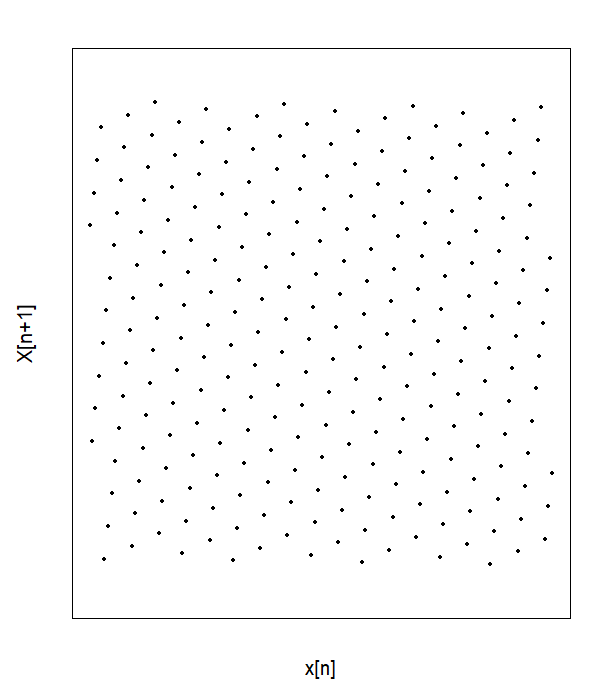
\includegraphics[width=\linewidth]{billder/spec_bad_lcg_2d.png}
		\caption{2D spectral test for LCG using bad parameters: $X_{n+1}=137\cdot X_{n}+187$ mod $256$}
		\label{fig:badspec2d}
	\end{minipage}\hfill
	\begin{minipage}{0.45\textwidth}
		\centering
		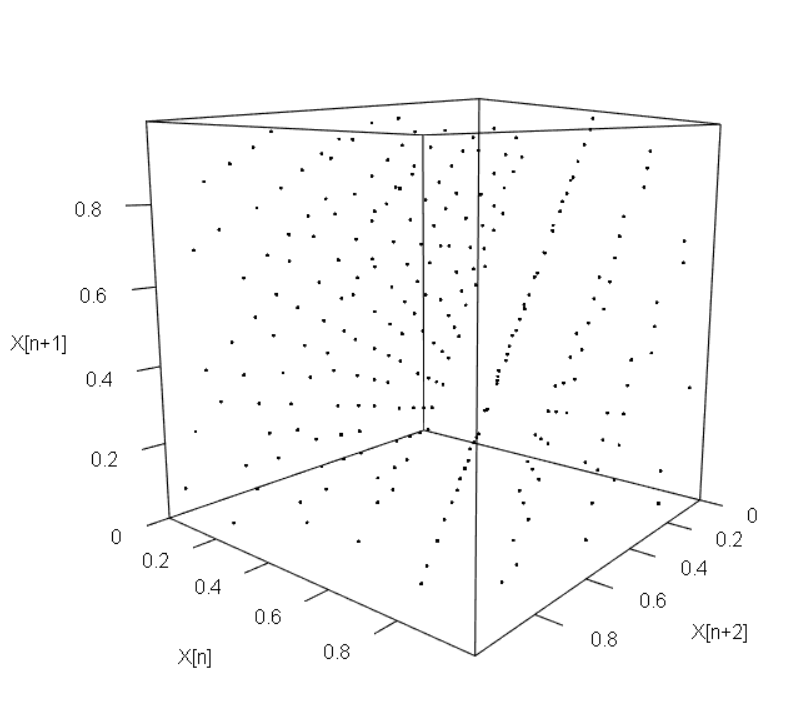
\includegraphics[width=\linewidth]{billder/spec_bad_lcg_3d.png}
		\caption{3D spectral test for LCG using bad parameters: $X_{n+1}=137\cdot X_{n}+187$ mod $256$}
		\label{fig:badspec3d}
	\end{minipage}
\end{figure}

%Spectral test good LCG
\begin{figure}
	\centering
	\begin{minipage}{0.45\textwidth}
		\centering
		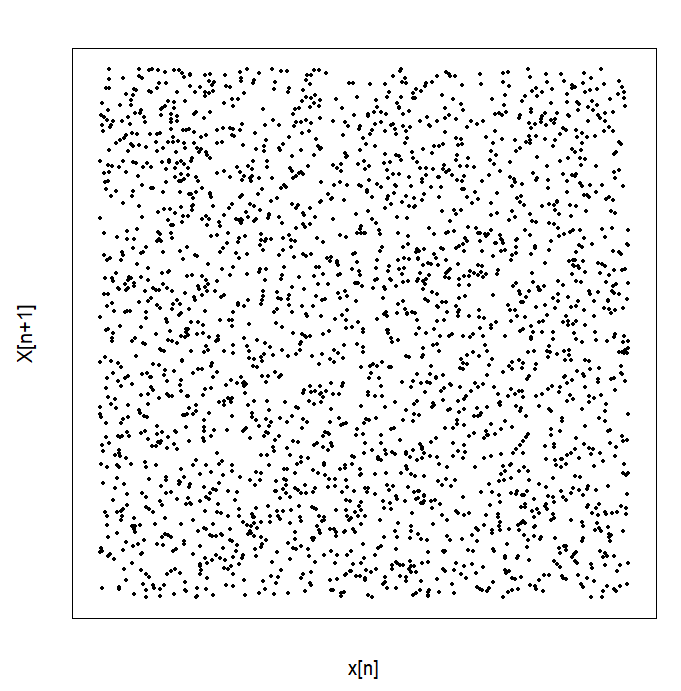
\includegraphics[width=\linewidth]{billder/spec_good_lcg_2d.png}
		\caption{2D spectral test for LCG using good parameters: $X_{n+1}=3 141 592 621\cdot X_{n}+1$ mod $2^{32}$}
		\label{fig:goodspec2d}
	\end{minipage}\hfill
	\begin{minipage}{0.45\textwidth}
		\centering
		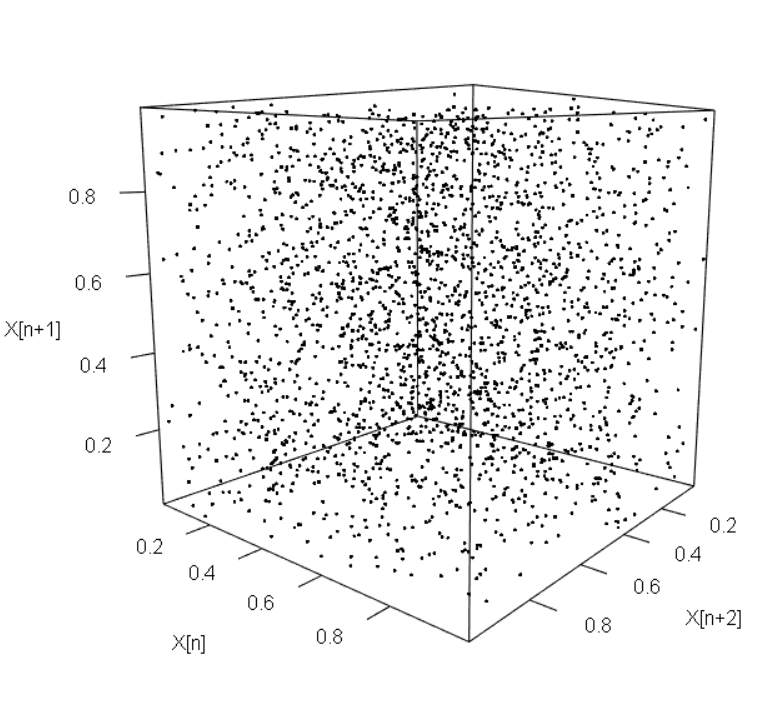
\includegraphics[width=\linewidth]{billder/spec_good_lcg_3d.png}
		\caption{3D spectral test for LCG using good parameters: $X_{n+1}=3 141 592 621\cdot X_{n}+1$ mod $2^{32}$}
		\label{fig:goodspec3d}
	\end{minipage}
\end{figure}

%Mersenne-Twister spectral tests
\begin{figure}
	\centering
	\begin{minipage}{0.45\textwidth}
		\centering
		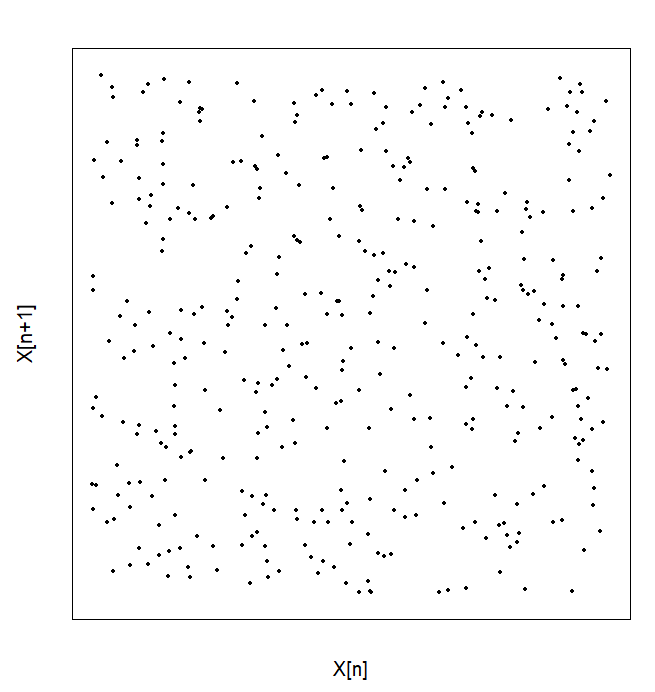
\includegraphics[width=\linewidth]{billder/ms_spec_2d.png}
		\caption{2D Spectral test for the PRNG Mersenne-Twister, in R}
		\label{fig:msspec2d}
	\end{minipage}\hfill
	\begin{minipage}{0.45\textwidth}
		\centering
		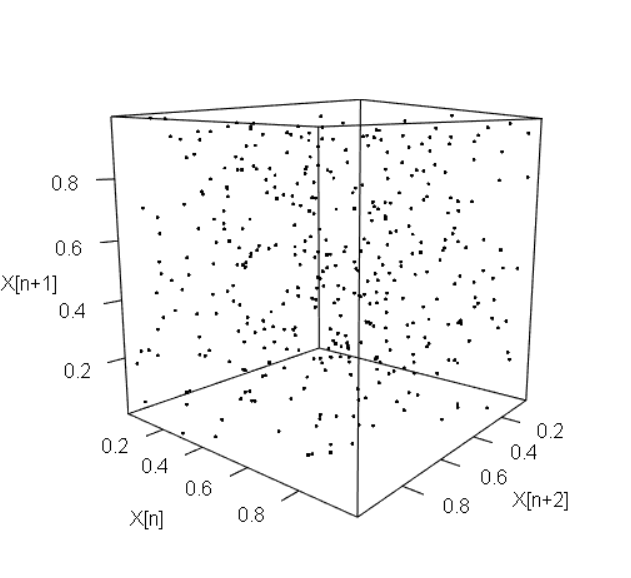
\includegraphics[width=\linewidth]{billder/ms_spec_3d.png}
		\caption{3D Spectral test for the PRNG Mersenne-Twister, in R}
		\label{fig:msspec3d}
	\end{minipage}
\end{figure}

	\newpage
	\subsection{The Bootstrap with the Monte Carlo Principle}
	\subsection{Monte Carlo Bootstrap}
The following mathematical theory is based on the book, "Mathematical Statistics with Resampling and R" (Chihara \& Hesterberg). The bootstrap is a procedure that uses a given sample to create a new distribution, called the bootstrap distribution. To find the bootstrap distribution, other samples are drawn from the original sample; in that way, it is a tool for resampling. The bootstrap distribution is used to approximate the sample distribution of a specific statistic $\theta$. For most statistics, bootstrap distributions approximate the spread, bias, and shape of the actual sampling distribution. The statistic could for example be the mean. To create the bootstrap distribution of the mean, bootstrap samples are drawn from the original sample, and then the mean is calculated for each resample. In other words, the original sample is now treated as the population. If the statistic tested is the mean, then the bootstrap distribution of the mean will look approximately like the sampling distribution of the mean and have almost the same spread and shape. However, note that the mean of the bootstrap distribution will be the same as the original sample and not the population. \newline
So, the idea of the bootstrap is that the original sample approximates the population. Therefore, resamples of the original sample would approximate the same as taking more samples from the population. That is indeed the concept of resampling.

\subsubsection{Resampling}
Resampling is a method in statistics used to estimate variability or improve model performance. In simple terms, resampling is creating new samples from existing data. There are different methods for resampling, one of them being bootstrapping. Bootstrapping is resampling with replacement. That means, when new samples are simulated, the same  data point can be chosen multiple times, because when it is selected from the original sample, it is put back before simulating the next sample. That way, the number of observations $n$ is always the same, but some data points might be chosen multiple times and others not at all.

\subsubsection{Method}
As previously mentioned, the principle of the bootstrap is to use a sample as an approximation of the population. From the samples, bootstrap samples are generated through resampling. The notation $*$ indicates a bootstrap sample. For every bootstrap sample, a statistic noted as $\hat{\theta}^*$ or $\overline{x}^*$ is calculated. The spread of the calculated $\hat{\theta}^*$ is defined as the bootstrap distribution.\newline

\noindent Bootstrapping is also used for confidence intervals for a population parameter $\theta$. If the values of the bootstrap distribution are known, it is possible to determine the confidence intervals by calculating the wanted percentiles. Typically a 95\% confidence interval is calculated, which is done by calculating the 2.5\% and 97.5\% percentile. This is called the bootstrap percentile confidence interval.

\subsubsection{Monte Carlo Principle}
In the bootstrap method with $n$ observations, there would theoretically be $\binom{2n-1}{n}$ different bootstrap samples. For large values of $n$, there would be a large amount of possible bootstrap samples. Therefore, it can be impractical or even impossible to generate all of them. To address this, the Monte Carlo Principle is applied, which means not every bootstrap sample has to be calculated to give precise results. Instead, a random amount of bootstrap samples is generated to approximate the distribution of the statistic of interest. Theory says that for "quick-and-dirty" resampling results 1000 samples should at least be made, but to ensure precise results, 10.000 samples or more are needed.

\subsubsection{Parametric and nonparametric bootstrap}
There are two types of bootstrapping: parametric and nonparametric. Parametric bootstrapping is when an assumption is made about the population's distribution. For example, assuming the data follows a normal distribution, then the parameters are estimated from that model, and new samples are generated by simulating data from the fitted distribution. Nonparametric bootstrapping is the opposite, when there are no assumptions made about the population's distribution. It resamples from the observed data with replacement and hereby treats the empirical distribution as an estimate for the population. In this project, the focus will be on the nonparametric bootstrap, because that is the one used. \newline

\noindent For the nonparametric bootstrap $\hat{F}(x)$ is the empirical cumulative distribution function, given by:
\begin{equation}
\hat{F}(x)=\frac{1}{n}(m\leq x).
\end{equation}
In addition to this, the nonparametric bootstrap also has an empirical probability mass function $\hat{f}(s)$, given by:
\begin{equation}
	\hat{f}(s)=\frac{1}{n}(m=s).
\end{equation}
In both cases $m$ represents the observed sample, and $n$ is the sample size. Each observation is assigned a probability of $\frac{1}{n}$ to be selected as a bootstrap sample. The  cumulative distribution $\hat{F}(x)$ tells the proportion of values in the sample that are less than or equal to the value $x$. The probability mass function $\hat{f}(s)$ gives the frequency of the value $s$ in the sample. The advantage of this method is that it is based on the sample, without knowing the distribution of the population. No assumptions are made, the data tells what it can, and no bias is introduced based on wrong assumptions.
	\newpage
	\subsection{metrics}
	To evaluate the quality of a regression model, various metrics are used. Each metric provides a score that reflects the reliability of the model's predictions.

Metrics are measures used to evaluate how well a model performs. Metrics assess the accuracy of the model’s predictions compared to actual values. Common metrics like R² and MBE help determine how closely predictions match real outcomes, while others like bias and variance reveal systematic errors and model stability. Metrics help model selection and improvement by providing objective feedback on performance. They’re essential for comparing models, detecting underfitting or overfitting, and ensuring predictions are reliable for real-world use.
\\\\

\subsubsection{R-Squared}
% What is it?
The $R^2$ (coefficient of determination) measures how much better the model predicts outcomes compared to simply using the mean. It is calculated using the Total Sum of Squares (TSS) and the Sum of Squared Errors (SSE) with this formula: 
$$R^2=1-\frac{\text{SSE}}{\text{TSS}}$$

TSS explains how much the values of a dataset vary from the mean and is calculated by: 
$$\sum_{j=1}^{n}(A_j - \bar{A})^2,$$
where $A_j$ is the actual value and $\hat{A}$ is the mean of all actual values.
\\\\

\noindent The SSE is how far the predictions from the model are from the actual values and is calculated by:
$$\sum_{j=1}^{n}(P_j - A_j)^2,$$
where $\hat{A}$ is the predicted value from the model, $P_{j}$ is the predicted value, $A_{j}$ is the actual value, and $n$ is the number of observations \cite{metrics}. The errors are squared to make all values positive, highlight larger mistakes more strongly, and stay consistent with how variance is calculated in statistics.
\\\\
% Interpretation
$R^2$ explains how much of the variance explained by the model. The value of $R^2$ typically lies in the range $0 \leq R^2 \leq 1$, where 0 means that the model explains none of the variance, a value of 1 would mean that the model explains all the variance, while 0.5 means that the model explains 50\% of the variance. If the $R^2$-value is negative, it means that the model is performing so poorly that it would be better to simply predict the mean for all observations.

\noindent Although widely used, the $R^2$-score should not be relied upon as the only metric of model performance due to several shortcomings. Primarily, it evaluates the proportion of variance in the dependent variable explained by the model, but does not reflect the accuracy of individual values. As a result, a model can achieve a high $R^2$ despite making major errors on specific data points. In addition, $R^2$ is vulnerable to overfitting, especially when the model becomes overly complex and starts fitting the noise in the data instead of underlying trends. Another critical issue is that $R^2$ does not adjust for the number of predictors in the model. It will never decrease when more features are added, even if those features are irrelevant. For a more reliable assessment, alternative metrics should be used alongside $R^2$ to evaluate a regression model. 
\newpage

\subsubsection{Mean Bias Error}
Mean Bias Error (MBE) is a metric that measures the average difference between the actual values and the model's predictions. Unlike other metrics, MBE does not emphasize the magnitude of the error but instead indicates whether the model systematically overestimates or underestimates, revealing potential bias in the predictions.

The formula for MBE is:

$$\text{MBE}=\frac{1}{n}\sum_{j=1}^{n}(e_{j}).$$

\noindent Here $e_{j}=A_{j}-P_{j}$, again $P_{j}$ is the predicted value, $A_{j}$ is the actual value, and $n$ is the number of observations \cite{metrics}.
\\\\

When interpreting MBE, there are three different cases to consider. If the $\text{MBE}\geq 0$, the model tends to over-predict the values compared to the actual values. If the $\text{MBE}\leq0$, the opposite is the case, and the model tends to under-predict the values. If the $\text{MBE}\approx0$ there is no consistent bias in either direction.
\\

\noindent The MBE measures the bias of the model, whether it tends to predict values that are generally too high or too low compared to the actual values. This means that we cannot use MBE to estimate the size of the error or the overall quality of the model. If two actual values are $100$ and the model predicts $120$ and $80$ the error calculated with $\hat{y}-y$ is $+20$ and $-20$. Because the absolute or squared values are not used, these errors will cancel each other out. Therefore, the size of the error is not computed. Instead, to understand the size of the errors, Root Mean Square Error can be used, which penalizes large deviations more heavily.

\newpage

\subsubsection{Root Mean Square Error}   

Root Mean Square Error (RMSE) is a metric used to evaluate regression models. It measures the average size of prediction errors. Since it squares the errors, it punishes larger errors more than smaller ones, which is useful if the objective is to emphasize the impact of larger deviations of the actual values.
\\
The formula for RMSE:
$$\text{RMSE}=\sqrt{\frac{ \sum_{j=1}^{n} e_j^2 }{n}}.$$
As before, here $e_{j}=A_{j}-P_{j}$, where $P_{j}$ is the predicted value, $A_{j}$ is the actual value, and $n$ is the number of observations \cite{metrics}.
\\ The idea is to find the error by subtracting the actual value from its prediction, square the error so negatives and positives do not cancel out (like in MBE) and large errors will stand out. Then the average of all squared errors is found, and the square root is taken to bring the result back to the original scale. 
\\

\noindent The RMSE is always a non-negative number, and the closer RMSE is to 0, the better the model is performing. The scale and unit of RMSE is the same as the target variable. So, if the data is about 'Miles Per Gallon', a RMSE of 2 means that the predictions of the model are 2 miles off, on average. Therefore, RMSE is most useful when the objective is comparing different models on the same dataset, or at least on datasets with the same scale, and in the same units. This also means an RMSE of 5 can be great if the values of the target variable range from 1-1000, but awful if the range is 1-10. Like the other metrics, RMSE should be used alongside other metrics to provide a more complete picture of the model’s performance. RMSE does not explain why a model performs well or poorly. To understand why a model performs poorly, bias-variance decomposition can be used to split error into systematic bias and model instability.
\newpage

\subsubsection{Bias-Variance}
To understand the sources of error in a model’s predictions, the bias-variance decomposition framework helps explain errors in a model’s predictions. Bias measures how far, on average, the model's predictions are from the true values. Variance describes how sensitive the model is to changes in the training data; it measures how much the model’s predictions vary when trained on different datasets. 

The ideal case is when both bias and variance are low, meaning the model is both accurate and stable. This framework is especially useful for diagnosing underfitting, which is caused by high bias, and overfitting, which is caused by high variance. By examining both bias and variance, the decomposition helps in understanding the trade-off between model complexity and generalization.

\subsubsection{Variance}
The variance of a model, for a single input, can be calculated using this formula:
$$
\text{Var}[\hat{f}(x)] = \frac{1}{M} \sum_{j=1}^{M} (\hat{f}_j(x) - \overline{\hat{f}}(x))^{2}.
$$

Where:
\begin{itemize}
	\item $M$ is the number of models or simulations,
	\item $\hat{f}_j(x)$ is the prediction by model $j$ at input $x$,
	\item $\overline{\hat{f}}(x)$ is the mean prediction across all $M$ models at input $x$.
\end{itemize}

This formula measures how much predictions vary at a specific input $x$ across multiple model runs. To calculate the overall variance across the input space, the average of the variances at all test inputs is taken:

$$
\text{Overall Model Variance} = \frac{1}{n} \sum_{i=1}^{n} \text{Var}[\hat{f}(x_i)].
$$

This overall measure is beneficial because it captures how the model’s prediction variability behaves across the entire dataset, rather than at just one point. A model with high variance is likely too complex and sensitive to the noise in the data.

\subsubsection{Bias}
Bias measures how far the model’s average prediction is from the true value. Since bias can be positive or negative, it is typically squared to focus on its magnitude. The squared bias for a specific input $x$ is calculated as:

$$
\text{Bias}^2(x) = (\overline{\hat{f}}(x) - f(x))^{2}.
$$

The overall squared bias across all inputs is calculated by averaging over the test set:

$$
\text{Bias}^2 = \frac{1}{n} \sum_{i=1}^{n} (\overline{\hat{f}}(x_i) - f(x_i))^{2}.
$$

High bias typically indicates that the model is too simple to capture the underlying structure of the data, resulting in systematic under- or over-prediction.



\subsubsection{Confidence Intervals}
Confidence intervals are used in model evaluation to judge the stability and reliability of a model's estimations. Unlike the previously mentioned metrics, confidence intervals do not provide a single number, but instead a range within which the true parameter value is likely to lie, given a specified level of confidence. The level of confidence is typically 95\%.

By comparing overlap and width of the confidence intervals across different models, it is possible to assess which model generates the best estimates, based on consistency and reliability.
	\newpage
	\subsection{Problem Statement}
	\label{sec:PBS}

The validity and correctness of a regression model build upon the ordinary least squares method relies on key assumptions to be fulfilled, specifically in context of this project. Here, the key assumption in focus is homoscedasticity (constant variance of errors). This assumption is essential for reliable statistical inference and parameter estimation. As established in section 3.6.5.1, when the assumption is not upheld, the results, such as confidence intervals and hypothesis testing, can be misleading.\\
The assumption of homoscedasticity may not always be upheld in the real world, so this project will explore Monte Carlo Bootstrapping as a resampling method that can overcome violations in regression assumptions and how this method can offer more reliable statistical results. We will test the method on generated data, where we can manipulate the data, so there is heteroscedasticity, and therefore test, if Monte Carlo Bootstrapping can help with the issue of a violated assumption. 


\begin{itemize}
	\item How will breaking the assumption of homoscedasticity in a classical polynomial regression affect the performance of the model, and how can this be solved by using Monte Carlo Bootstrapping?
\end{itemize}

	\newpage
	%input{intro til data}
	%	\newpage
	
	%	\section{M	\section{intro til data}
		%	\onte Carlo Regression}
	%	\newpage
	
	%	

\section{montecarlo bootstrapping }

Monte Carlo bootstrapping is used to find the model for the mpg data. It starts by cleaning the data, then selecting the numeric columns, and defining the Monte Carlo bootstrapping function. After that, it defines the polynomial regression function using mpg as the dependent variable. Next, it defines the simulation function using clusters, thereby speeding up the computation time with the doParallel library. After defining the run simulation function, it runs the simulation with the set seed, simulation number, and sample size of the Monte Carlo bootstrapping method.

After that, it creates histograms of the simulation results. It calculates the mean result of the coefficients, and using these means, it calculates a new regression model and the R-squared of the new average model. Finally, it makes a scatter plot showing the final regression model results versus the results from the actual data set.
%\lstinputlisting[language=R, caption=montecarlo bootstrapping]{kode/montecarlo bootstrapping.R}

\begin{figure}[h] 
	\centering
	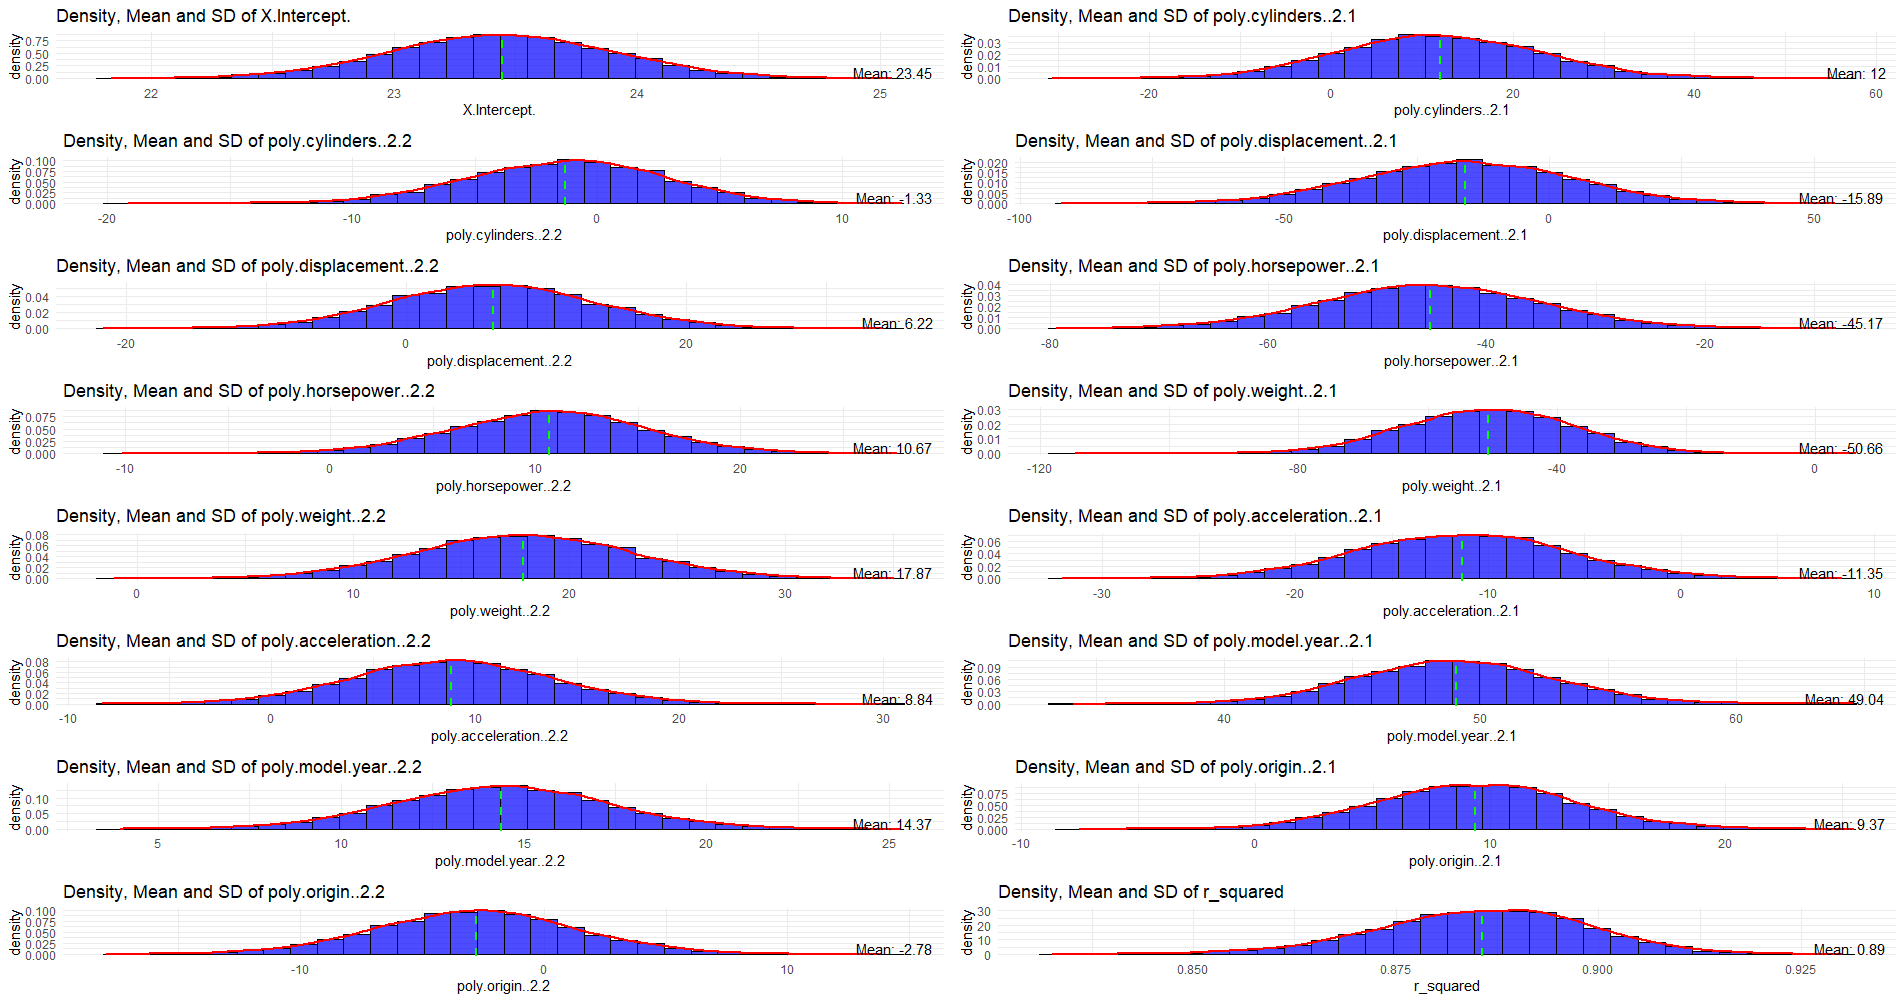
\includegraphics[width=14cm]{billder/10.png}
	\caption{AQI gennem årene.}
	\label{fig:j06}
\end{figure}

%\begin{figure}[h] 
%	\centering
%%	\caption{AQI gennem årene.}
%	\label{fig:j06}
%\end{figure}
	
	
	%	\section{super syntetisk}
	%	\section{super syntetisk }

To show the consequences of violating the assumption of homoscedasticity, a dataset is generated with and without homoscedasticity. It starts with generating four normally distributed independent variables using a random number generator. Then, the dependent variable is generated as a function of the four independent variables. A regression model is fitted, and the model is tested. After this, homoscedasticity is violated by adding an error term that scales with the dependent variable. The model is tested again, and it becomes apparent what the consequences of violating the assumption of homoscedasticity are.

\lstinputlisting[language=R, caption=super syntetisk data]{C:/Users/Jonathan/Documents/GitHub/P2/R kode/super syntetisk data_.R}



\begin{figure}[h] 
	\centering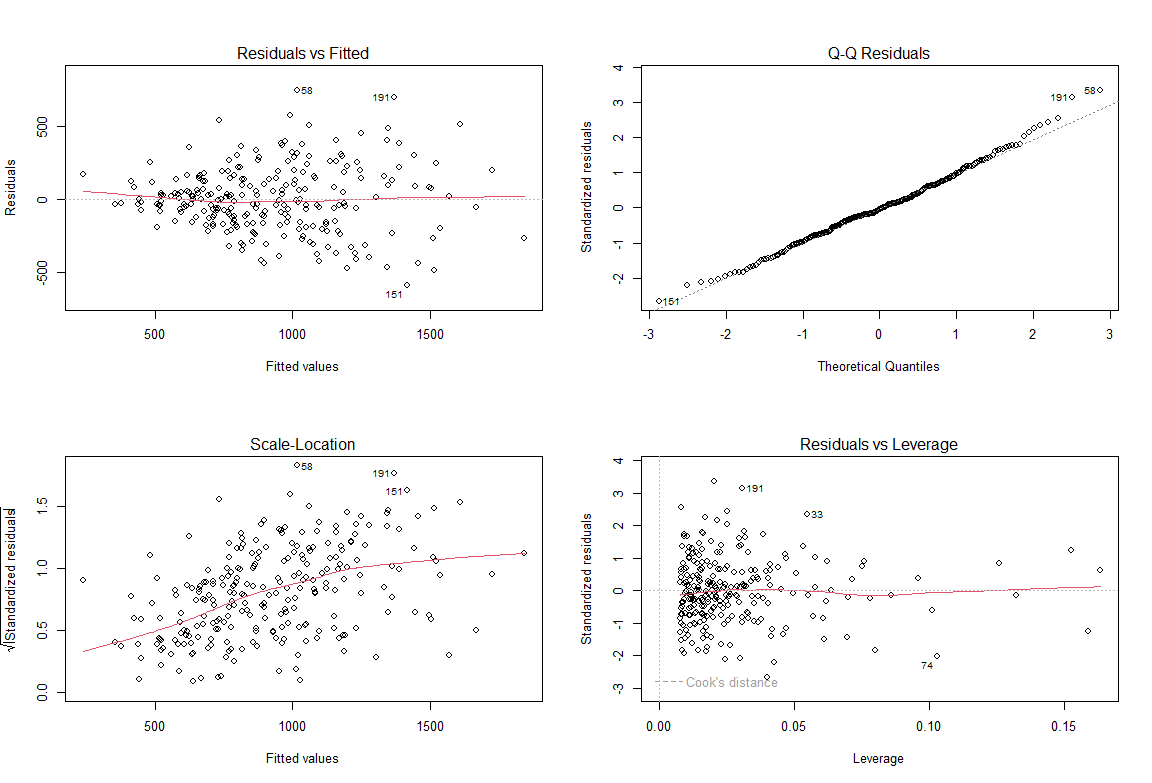
\includegraphics[width=14cm]{p2/4.png}
	\caption{residualplot}
	\label{fig:j06}
\end{figure}

\begin{figure}[h] 
	\centering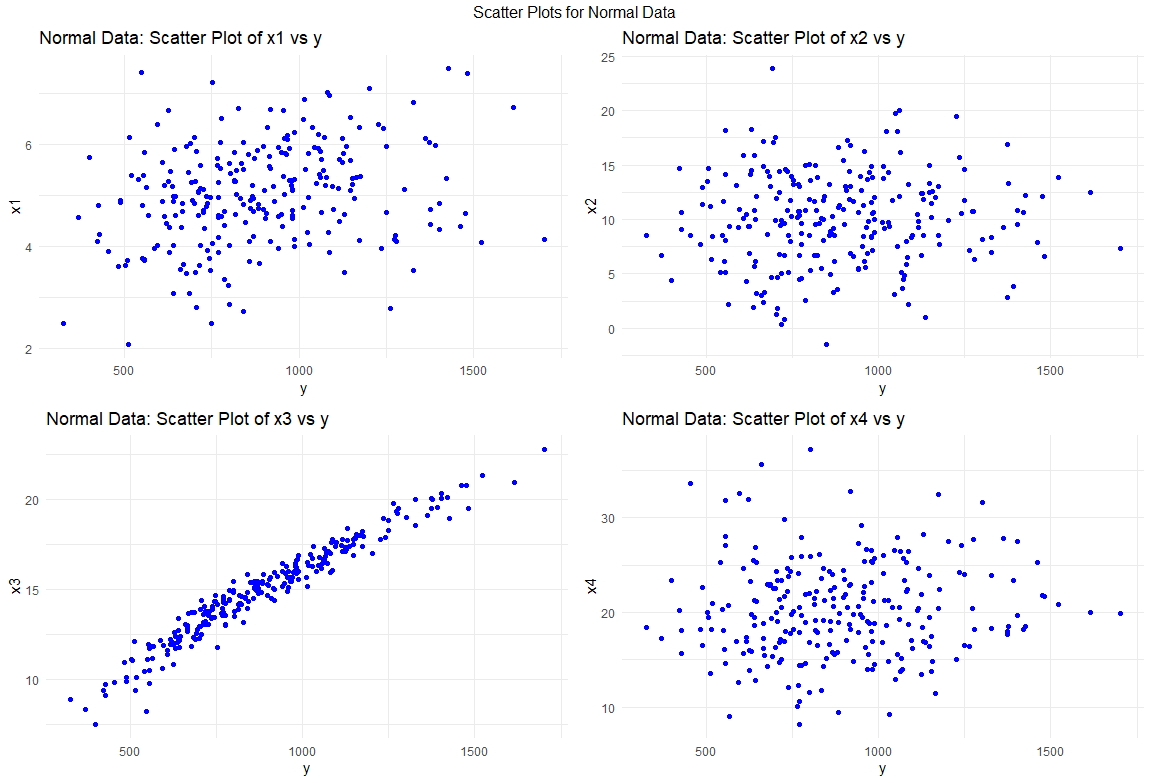
\includegraphics[width=14cm]{p2/5.png}
	\caption{scatterplot.homo}
	\label{fig:j06}
\end{figure}

\begin{figure}[h] 
	\centering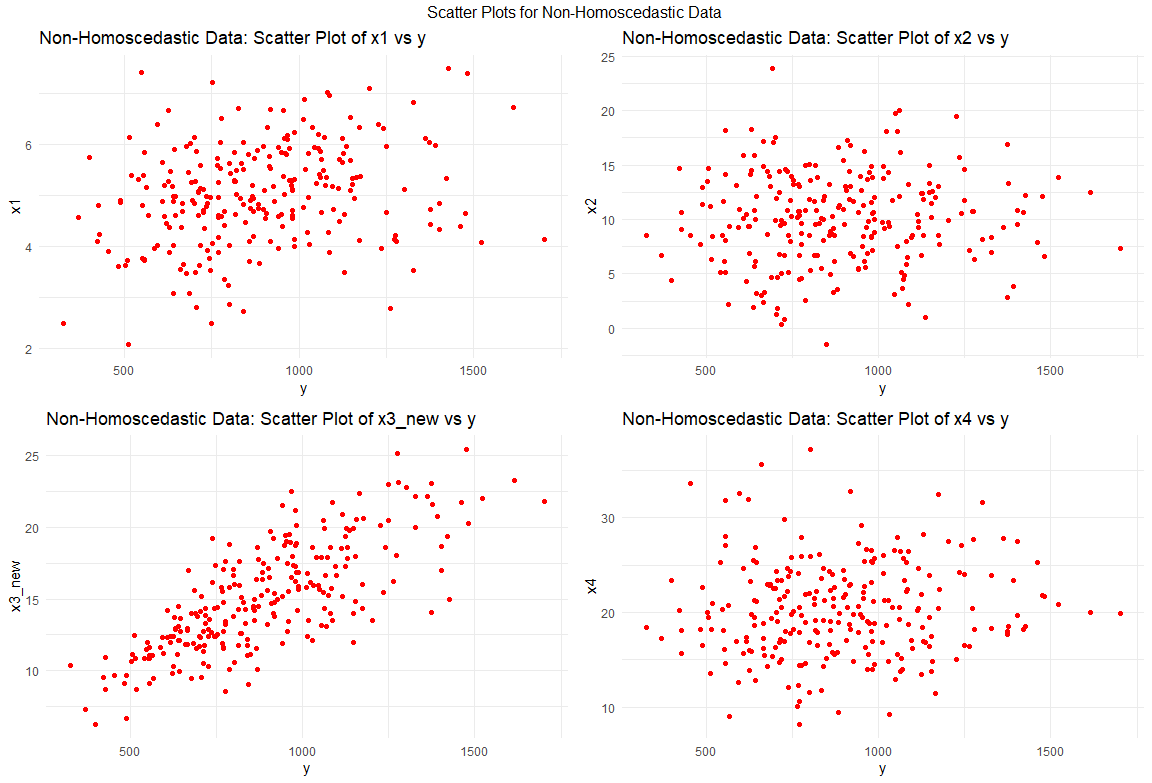
\includegraphics[width=14cm]{p2/6.png}
	\caption{scatterplot.hetro}
	\label{fig:j06}
\end{figure}

\begin{figure}[h] 
	\centering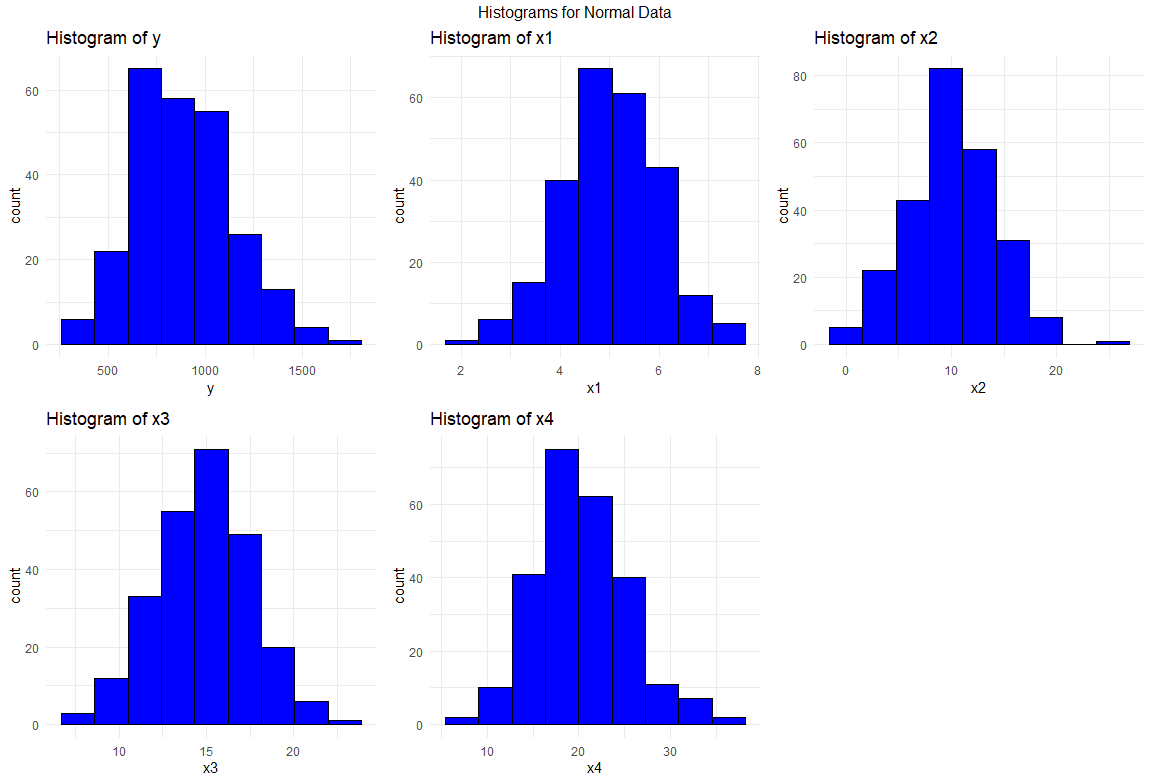
\includegraphics[width=14cm]{p2/7.png}
	\caption{his.homo}
	\label{fig:j06}
\end{figure}

\begin{figure}[h] 
	\centering
	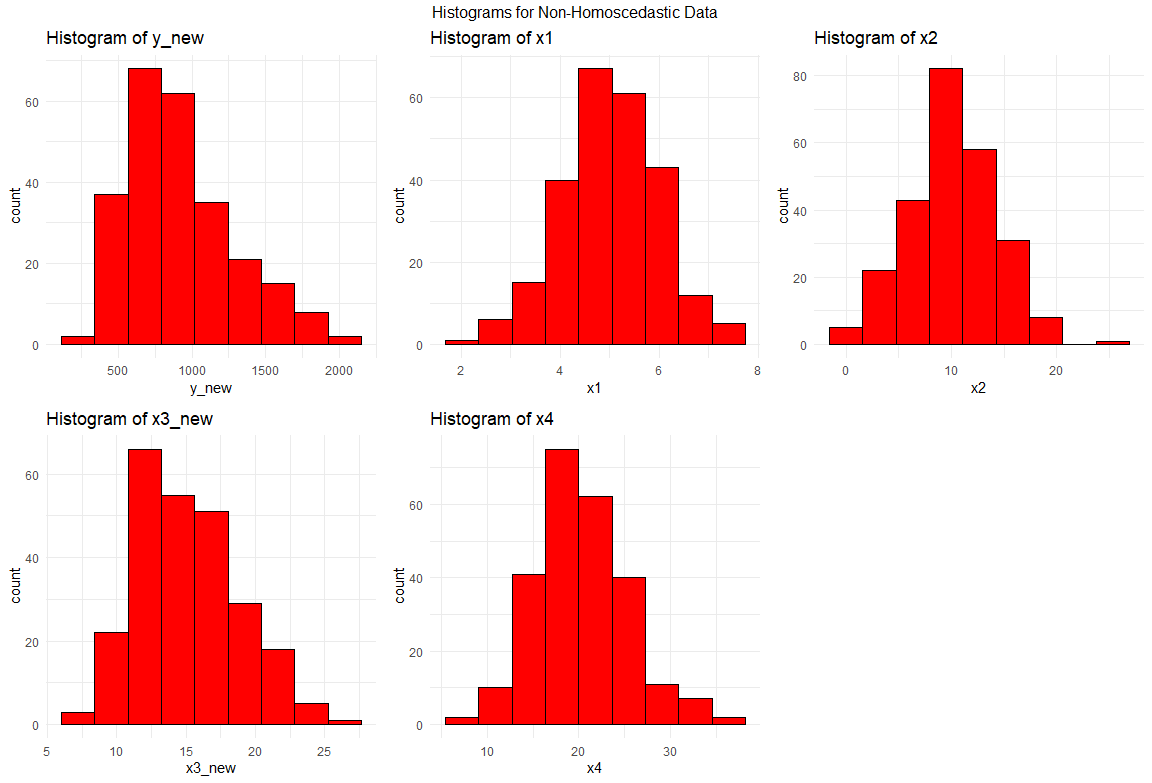
\includegraphics[width=14cm]{p2/8.png}
	\caption{his.hetro.}
	\label{fig:j06}
\end{figure}

	%	\newpage
	
	
	\section{Comparison between Regressions}
	

To understand how assumption violations affect classical polynomial regression, we begin by generating synthetic data using a random number generator. First, four independent variables are created, each normally distributed with known standard deviations. Then, the dependent variable is generated as a function of these four independent variables. This synthetic dataset initially satisfies all the assumptions required for ordinary least squares (OLS) regression.
\\\\
Next, an error term is added that scales with the dependent variable. This introduces heteroscedasticity meaning the error variance is no longer constant thereby violating the assumption of homoscedasticity. This step is done deliberately to ensure that this is the only assumption being violated, so any observed effects on the model can be attributed specifically to this violation.
\\\\
The dataset is then split into training and test sets, with $80\%$ used for training and the remaining $20\%$ for testing. A standard linear polynomial regression model is fitted to the training data. The mean bias error and root mean squared error (RMSE) calculated are useing the testdata and standard error, and confidence intervals for the coefficients are calculated all this is to evaluate the model's performance.
\\\\
Following this, a bootstrap is performed by resampling the training data 10000 times. For each resampled dataset, a linear polynomial model is fitted. The coefficients from each model are stored in a new data frame, and predictions are made on the test data and also stored in the dataframe. These predictions are then compared to the actual test values to compute the mean bias error and RMSE and the coefficients are used the calculated the standard error and confidence intervals of the coefficients for the bootstrap models.
\\\\
Comparing the results of the two models shown in Table 2, the Mean Bias Error (MBE) of the OLS model is -539, indicating that it tends to underpredict the actual values. In contrast, the bootstrap model has an MBE of 22, suggesting a slight overprediction. The smaller absolute bias of the bootstrap model indicates improved accuracy. This is further supported by the Root Mean Square Error (RMSE), where the OLS model scores 1921 compared to the bootstrap model’s 1377. This substantial difference reinforces the conclusion that the bootstrap model provides more accurate predictions.
\\\\
When comparing the standard errors of the estimated coefficients, the OLS model appears to have lower standard errors. However, it is important to note that these may not be reliable due to the violation of the homoscedasticity assumption. In such cases, the standard errors from OLS can be misleading. In contrast, the bootstrap standard errors are derived from the empirical distribution of the data and are therefore more representative of the true variability. As a result, the confidence intervals produced by the OLS model may not be trustworthy, while those from the bootstrap model better reflect the uncertainty in the estimates showing a false sense of predictability. Overall, the bootstrap approach demonstrates superior predictive performance and more robust inference under assumption violations.
\\



\begin{table}
	\centering
	\caption{Opdateret Sammenligning af OLS og Bootstrap modeller}
	\begin{tabular}{lcc}
		\hline
		& \textbf{OLS} & \textbf{Bootstrap} \\
		\hline
		\textbf{MBE} & -539.4769 & 22.2755 \\
		\textbf{RMSE} & 1921.0420 & 1377.4900 \\
		\hline
		\textbf{Std. Error} \\
		\hline
		Intercept & 478.4811 & 540.9184 \\
		$I(x1^2)$ & 1.4306e-03 & 3.2636e-03 \\
		$I(x2^3)$ & 3.0470e-07 & 9.8684e-07 \\
		$I(x3^4)$ & 7.5112e-12 & 5.1212e-09 \\
		$I(x4^5)$ & 2.4766e-13 & 4.2884e-12 \\
		\hline
		\textbf{Coefficient (95\% CI)} \\
		\hline
		Intercept & [2854.183 , 4796.919] & [2443.400 , 4556.982] \\
		$I(x1^2)$ & [0.0004 , 0.0062] & [0.0023 , 0.0128] \\
		$I(x2^3)$ & [-1.06e-06 , 1.80e-07] & [-2.70e-06 , 6.24e-07] \\
		$I(x3^4)$ & [3.34e-11 , 6.39e-11] & [4.33e-11 , 1.20e-08] \\
		$I(x4^5)$ & [-3.48e-12 , -2.47e-12] & [-4.23e-12 , 8.08e-12] \\
		\hline
	\end{tabular}
\end{table}
	\newpage
	
	\section{Discussion}
	\subsection{Assumption Violations and Implications}
The objective of this prroject has been to investigate how breaking key asssumptions, like homoskcedasticity and multicollinarity, impacts the performance of classical polynomial regression models, and how Monte Carlo bootstrapping can offer a more reliable alternative. Synthetic data were used to deliberately violate the assumption of homoscedasticity while controlling other variables. This allowed for a focused analysis of how non-constant error variance influences model accuracy and inference.

\noindent Violating the homoscedasticity assumption was shown to significantly distort the performance of the ordinary least squares (OLS) model. The resulting regression had a notably high Root Mean Square Error (RMSE) and a strong negative bias, indicating that such violations can invalidate the statistical conclusions. 

\subsection{Bootstrapping as a Solution}
To address these assumption violations, bootstrapping was applied as a nonparametric resampling method. Since it is based on the empirical distribution of the data rather than relying on theoretical assumptions, bootstrapping offers a flexible alternative to OLS.

\noindent The results support this effectiveness. The bootstrap model produced a substantially lower RMSE (1377 vs. 1921) and a near-zero MBE (22 vs. -539), indicating more accurate and less biased predictions. This suggests that bootstrapping can successfully mitigate the effects of assumption violations and improve model robustness.

\subsection{Alternative Approaches and their Limitations}
Several alternative methods can be used to handle heteroscedasticity. One is Weighted Least Squares (WLS), which adjusts for variable variance by assigning different weights to each data point. However, determining appropriate weights is often computationally intensive and can introduce more uncertainty, since estimated weights are used. Additionally, it complicates model interpretation, as results depend on the weighting scheme.

\noindent Transforming the data with techniques like log or square root transformations, is another common approach. While these can sometimes stabilize variance, they do not consistently resolve assumption violations. In some cases, they may even worsen heteroscedasticity. Again, interpretation becomes more difficult, as the model no longer operates on the original scale of the variables.


\subsection{Strengths and Limits of Bootstrapping}
For these reasons, bootstrapping remains widely used despite its computational demands. Because it draws directly from the empirical distribution, bootstrapping makes fewer theoretical assumptions and often yields more robust results when an assumption like homoscedasticity is violated. However, it is not without limitations. The number of resamples must be chosen carefully to balance precision and efficiency. In the case of parametric bootstrapping, the method still relies on the assumption that the sample accurately represents the population. Another limitation comes from the use of the mean to estimate parameters, which can make bootstrap models sensitive to outliers and lead to distorted results if such anomalies are not properly addressed.

\noindent In summary, while several methods exist to address assumption violations in regression, bootstrapping, through this project, proved very effective. It provided more accurate predictions, reduced bias, and more reliable confidence intervals under heteroscedastic conditions. Although not without limitations, its empirical and assumption-light approach makes it a preferable method, when assumptions are violated.
	\newpage
	
	\section{Conclusion}
	\input{Conclusion}
	\newpage
	
	\section{Litteratur}
	
	\section{latextables}
	\newpage
	
	\bibliographystyle{plain}
	\bibliography{references}
	
\end{document}